\documentclass[french,12pt,a4paper]{book}
\usepackage{gensymb} 
\usepackage[utf8]{inputenc}
\usepackage[T1]{fontenc}
\usepackage[english]{babel}
\usepackage[default, scale=.95]{opensans} % police Open Sans
\usepackage{fontawesome}
\usepackage{amsmath}
\usepackage{amsfonts}
\usepackage{fancyhdr}
\usepackage{amssymb}
\usepackage{xcolor} % où color selon l'installation
\definecolor{Prune}{RGB}{99,0,60} % l14-33 : couleurs de la charte graphique upsaclay
\definecolor{B1}{RGB}{49,62,72} 
\definecolor{C1}{RGB}{124,135,143}
\definecolor{D1}{RGB}{213,218,223}
\definecolor{A2}{RGB}{198,11,70}
\definecolor{B2}{RGB}{237,20,91}
\definecolor{C2}{RGB}{238,52,35}
\definecolor{D2}{RGB}{243,115,32}
\definecolor{A3}{RGB}{124,42,144}
\definecolor{B3}{RGB}{125,106,175}
\definecolor{C3}{RGB}{198,103,29}
\definecolor{D3}{RGB}{254,188,24}
\definecolor{A4}{RGB}{0,78,125}
\definecolor{B4}{RGB}{14,135,201}
\definecolor{C4}{RGB}{0,148,181}
\definecolor{D4}{RGB}{70,195,210}
\definecolor{A5}{RGB}{0,128,122}
\definecolor{B5}{RGB}{64,183,105}
\definecolor{C5}{RGB}{140,198,62}
\definecolor{D5}{RGB}{213,223,61}
\usepackage{mdframed}
\usepackage{multirow} %% Pour mettre un texte sur plusieurs rangées
\usepackage{multicol} %% Pour mettre un texte sur plusieurs colonnes
\usepackage{scrextend} %Forcer la 4ème  de couverture en page pair
\usepackage{tikz}
\usepackage{graphicx}
\usepackage[absolute]{textpos} 
\usepackage{colortbl}
\usepackage{array}
\usepackage{geometry}
\usepackage{titlesec}
\usepackage{tocloft}
\usepackage{hyperref}
\usepackage{csquotes}
\usepackage[backend=biber,style=alphabetic]{biblatex}
\addbibresource{references.bib}
\usepackage[toc]{glossaries}
\newcommand{\trr}[1]{\trace \left[ #1 \right]}
\newcommand{\mean}[1]{\ensuremath{\langle {#1} \rangle}}
\newcommand{\Hil}{\ensuremath{\mathscr{H}}}
\newcommand{\id}{\ensuremath{\mathds{1}}}

\makeglossaries

\newacronym{epr}{EPR}{Einstein, Podolsky and Rosen}
\newacronym{chsh}{CHSH}{Clauser-Horne-Shimony-Holt}
\newacronym{sos}{SOS}{Sum-of-Squares}
\newacronym{CPTP}{CPTP}{completely-positive trace-preserving}

\newacronym{povm}{POVM}{positive-value operator measurement}
\newacronym{DIQKD}{DIQKD}{Device-Independent Quantum Key Distribution}
\newacronym{QKD}{QKD}{Quantum Key Distribution}

\newacronym{rl}{RL}{Reinforcement Learning}

\hypersetup{ % paramétrage couleur des liens hypertextes, toujours garder colorlinks=true
	colorlinks=true,
	linkcolor=black,
	urlcolor=purple}
 
\makeatletter
\renewcommand{\numberline}[1]{%
  \@cftbsnum #1\@cftasnum~\@cftasnumb%
}
\makeatother

\pagestyle{plain} % pour ne garder que les n°de page en milieu-bas et supprimer les indications de chapitre en marge haute

\usepackage{lipsum} % à retirer!!!
\begin{document}
	
	\begin{titlepage}
		
		%\thispagestyle{empty}
		
		\newgeometry{left=6cm,bottom=2cm, top=1cm, right=1cm}
		
		\tikz[remember picture,overlay] \node[opacity=1,inner sep=0pt] at (-13mm,-135mm){
\includegraphics{Logo/Frame-ups.pdf}};
		
		%*****************************************************
		%******** NUMÉRO D'ORDRE DE LA THÈSE À COMPLÉTER *****
		%******** POUR LE SECOND DÉPOT                   *****
		%*****************************************************
		
		\color{white}
		
		\begin{picture}(0,0)
			\put(-152,-743){\rotatebox{90}{\Large \textsc{THESE DE DOCTORAT}}} \\
			\put(-120,-743){\rotatebox{90}{NNT : 2020UPASA001}}
		\end{picture}
		
		%*****************************************************
		%**  LOGO  ÉTABLISSEMENT PARTENAIRE SI COTUTELLE
		%**  CHANGER L'IMAGE PAR DÉFAUT **
		%*****************************************************
		\vspace{-14mm} % à ajuster en fonction de la hauteur du logo
		%\flushright \includegraphics[scale=1]{logo2.png}
		
		%*****************************************************
		%******************** TITRE **************************
		%*****************************************************
		
		\flushright
		\vspace{30mm} % à régler éventuellement
		\color{Prune}
		\fontfamily{cmss}\fontseries{m}\fontsize{22}{26}\selectfont
		\Huge Device-independent certification: from foundations to applications \\
		
		\normalsize
		\color{black}
		\Large{\textit{Device-independent certification: Fondations et Applications}}\\
		%*****************************************************
		
		\fontfamily{fvs}\fontseries{m}\fontsize{8}{12}\selectfont
		
		\vspace{1.5cm}
		
		\normalsize
		\textbf{Thèse de doctorat de l'université Paris-Saclay} \\
		
		\vspace{6mm}
		
		\small École doctorale n\degree564 : physique en Île-de-France (PIF)\\
		\small Spécialité de doctorat: Physique\\
		\small Graduate School : Physique, Référent : Faculté des sciences d'Orsay \\
		\vspace{6mm}
		
		\footnotesize Thèse préparée à l’Institut de Physique Théorique (Université Paris-Saclay, CNRS, CEA) sous la direction de Nicolas Sangouard, directeur de recherche (CEA). \\
		\vspace{15mm}
		
		\textbf{Thèse soutenue à Paris-Saclay, le JJ mois AAAA, par}\\
		\bigskip
		\Large {\color{Prune} \textbf{Xavier VALCARCE}}
		
		%************************************
		\vspace{\fill} % ALIGNER LE TABLEAU EN BAS DE PAGE
		%************************************
		
		\bigskip
		
		\flushleft
		\small \textbf{Composition du jury}\\
		\vspace{2mm}
		\scriptsize
		\begin{tabular}{|p{7cm}l}
			\arrayrulecolor{Prune}
			\textbf{Prénom Nom} &   Président ou Présidente\\ 
			Titre, Affiliation & \\
			\textbf{Prénom Nom} &  Rapporteur \& Examinateur / trice \\ 
			Titre, Affiliation   &   \\ 
			\textbf{Prénom Nom} &  Rapporteur \& Examinateur / trice \\ 
			Titre, Affiliation  &   \\ 
			\textbf{Prénom Nom} &  Examinateur ou Examinatrice \\ 
			Titre, Affiliation   &   \\ 
			\textbf{Prénom Nom} &  Examinateur ou Examinatrice \\ 
			Titre, Affiliation   &   \\ 
			\textbf{Nicolas Sangouard} &  Directeur ou Directrice de thèse \\ 
			Titre, Affiliation   &   \\ 
			
		\end{tabular} 
		
	\end{titlepage}

\Ifthispageodd{\newpage\thispagestyle{empty}\null\newpage}{}
\thispagestyle{empty}
\newgeometry{top=1.5cm, bottom=1.25cm, left=2cm, right=2cm}
\fontfamily{rm}\selectfont

\lhead{}
\rhead{}
\rfoot{}
\cfoot{}
\lfoot{}

\noindent 
%*****************************************************
%***** LOGO DE L'ED À CHANGER IMPÉRATIVEMENT *********
%*****************************************************

\includegraphics[height=2.45cm]{Logo/logo_usp_PIF.png}
\vspace{1cm}
%*****************************************************
\fontfamily{cmss}\fontseries{m}\selectfont

\small

\begin{mdframed}[linecolor=Prune,linewidth=1]
	
	\textbf{Titre:} titre (en français)..................................................................................................................
	
	\noindent \textbf{Mots clés:} 3 à 6 mots clefs (version en français)
	
	\vspace{-.5cm}
	\begin{multicols}{2}
		\noindent \textbf{Résumé:}\lipsum[1-2] 
	\end{multicols}
	
\end{mdframed}

\vspace{8mm}

\begin{mdframed}[linecolor=Prune,linewidth=1]
	
	\textbf{Title:} titre (en anglais)..................................................................................................................
	
	\noindent \textbf{Keywords:} 3 à 6 mots clefs (version en anglais)
	
	\begin{multicols}{2}
		\noindent \textbf{Abstract:} \lipsum[1-2]
	\end{multicols}
\end{mdframed}

\titleformat{\part}[block]{\bfseries\Huge\color{Prune}\filright}{\thepart\ --\ }{.1ex}
{\vspace{0.1ex}
}
[\vspace{1ex}]

\titleformat{\chapter}[hang]{\bfseries\Large\color{Prune}}{\thechapter\ -}{.1ex}
{\vspace{0.1ex}
}
[\vspace{1ex}]
\titlespacing{\chapter}{0pc}{0ex}{0.5pc}

\titleformat{\section}[hang]{\bfseries\normalsize}{\thesection\ .}{0.5pt}
{\vspace{0.1ex}
}
[\vspace{0.1ex}]
\titlespacing{\section}{1.5pc}{4ex plus .1ex minus .2ex}{.8pc}

\titleformat{\subsection}[hang]{\bfseries\small}{\thesubsection\ .}{1pt}
{\vspace{0.1ex}
}
[\vspace{0.1ex}]
\titlespacing{\subsection}{3pc}{2ex plus .1ex minus .2ex}{.1pc}

\newcounter{article}
\newcommand{\article}[1]{%
  \par\refstepcounter{article}% Increase section counter
  \sectionmark{#1}% Add section mark (header)
  \addcontentsline{toc}{chapter}{\protect\numberline{Article \thearticle}#1}% Add section to ToC
  % Add more content here, if needed.
}
\frontmatter

\newgeometry{top=4cm, bottom=4cm, left=2cm, right=2cm}

\chapter{Acknowledgements}
\newpage

\tableofcontents

\newgeometry{top=4cm, bottom=4cm, left=4cm, right=4cm}

\printglossary[type=\acronymtype,title=Acronyms, toctitle=Acronyms]

\chapter{Thesis overview}

\section{Motivations and background}

\section{Summary of the contributions}

\chapter{Synthèse en français}

\section{Motivations et context}

\section{Résumé des contributions}

\chapter{Organisation of the manuscript}

\chapter{Publications}

This thesis is based on the following contributions.

\paragraph{Publications:}
\begin{enumerate}
	\item 
		\textit{What is the minimum CHSH score certifying that a state resembles the singlet?} \\
		Xavier Valcarce, Pavel Sekatski, Davide Orsucci, Enky Oudot, Jean-Daniel Bancal, and Nicolas Sangouard. \\
		\textit{Quantum}, volume 4, page 246.
	\item 
		\textit{Self-testing two-qubit maximally entangled states from generalized Clauser-Horne-Shimony-Holt tests} \\
		Xavier Valcarce, Julian Zivy, Nicolas Sangouard, and Pavel Sekatski. \\
		\textit{Phys. Rev. Research} 4, 013049.
	\item
		\textit{Device-independent quantum key distribution from generalized CHSH inequalities} \\
		Pavel Sekatski, Jean-Daniel Bancal, Xavier Valcarce, Ernest Y.-Z. Tan, Renato Renner, and Nicolas Sangouard. \\
		\textit{Quantum}, volume 5, page 444.
	\item 
		\textit{Automated design of quantum optical experiments for device-independent quantum key distribution}  \\
		Xavier Valcarce, Pavel Sekatski, Elie Gouzien, Alexey Melnikov, Nicolas Sangouard. \\
		\textit{Phys. Rev. A} 107, 062607.
\end{enumerate}

\paragraph{Codes:}
\begin{enumerate}
	\setcounter{enumi}{4}
	\item \textsc{QuantumOpticalCircuits.jl} --- Julia framework for the simulation of photonic circuits. \\
		\url{https://github.com/xvalcarce/QuantumOpticalCircuits.jl}
	\item \textsc{SPDCStats.jl} --- Julia package to compute statistics arising from a SPDC source and non photon-number resolving photodetectors. \\
		\url{https://github.com/xvalcarce/SPDCStats.jl}
\end{enumerate}


\mainmatter

\part{Self-testing for device-independent certification}

\chapter{Overview and definitions}

In this chapter we review the basis 

\section{Quantum Entanglement}

\section{Non-locality}

\subsection{Classical correlations}

\subsection{Non-local correlations}

\subsection{Bell inequality}

\section{Device-independent approach}

\section{Self-testing}

\chapter{Self-testing of the two-qubit maximally entangled state}

Two-qubit maximally entangled states are relevant to a few quantum information processing tasks.
In this chapter we study the self-test of such states in a fully device-independent scope, i.e. how to ensure that a two-qubit maximally entangled state is present in a system without making assumption on that state and on the measurements used to probe that state.
Specifically, we here present a self-test protocol based on the \acrshort{chsh} criterion, where a maximal \acrshort{chsh} score is the only requirement for the validity of the proof. Note that this approach differs slightly from the original method introduce in \cite{Mayers2004}.

\medbreak 

We consider a variation of a Bell game where Alice and Bob receive copies of an unknown state $\rho_{AB} \in \mathcal{L}(\mathscr{H}^A \otimes \mathscr{H}^B)$ from an unknown source.
Alice has access to the subsytem that lays in the Hilbert space $\mathscr{H}^A$ while Bob has access to the one in $\mathscr{H}^B$, both of unknown dimension.
To ease calculations, we can purify this shared state, without loss of generalities. 
Introducing the purification space $\Hil^C$, we have the pure shared state $\ket{\psi_{ABC}}\in \Hil^A \otimes \Hil^B \otimes \Hil^C$ which satisfies $\tr_C \left[\ket{\psi_{ABC}}\bra{\psi_{ABC}}\right] = \rho_{AB}$, where $\tr_C$ is the partial trace over the purification space.

Each party has a measurement device with two inputs, $x,y=\{0,1\}$, respectively corresponding to observables $A_x$ acting on $\mathscr{H}^A$, for Alice, and $B_y$ on $\mathscr{H}^B$, for Bob.
These measurements only have two possible outcomes $(a,b)=\pm1$.
From this Bell game, Alice and Bob will construct the correlation $P$ from the individual probabilities $p(ab|xy)$. 
It is solely from this correlation that we want to certify that $\rho_{AB}$ is a two-qubit maximally entangled state $\ket{\psi^{\text{target}}_{AB}}$.

Formally, a self-testing statement can be derived if for all the \textit{quantum realization} $\{\psi_{ABC},A_x,B_y\}$ compatible with the observed correlation $P$, there exists a local isometry $\Lambda = \Lambda_A \otimes \Lambda_B \otimes \id_C$ satisfying
\begin{equation}
	\Lambda [ \ket{00}_{A'B'} \otimes \ket{\psi}_{ABC}] = \ket{\psi^\text{target}_{A'B'}} \otimes \ket{\text{junk}}_{ABC}
	\label{eq:self-testing_statement}
\end{equation}
where $A'$ and $B'$ are ancilliary systems owned by Alice and Bob, respectively, and that are used to \textit{extract} the target state.
The rest of this chapter explains how to obtain this statement for two-qubit maximally entangled states.

\medbreak

As stated in the previous chapter, the \acrshort{chsh} inequality 
\begin{equation}
	S = \left | \mean{A_0 B_0} + \mean{A_0 B_1} + \mean{A_1 B_0} - \mean{A_1 B_1}  \right | \leq 2
\end{equation}
is maximally violated for a \acrshort{chsh} score of $2\sqrt{2}$, and such a score can be obtain from a maximally entangled two-qubit state and anticommuting measurements. 
Conversely, it was proven that a score of $2\sqrt{2}$ can only be reached by a maximally entangled state, and for anticommuting measurements~\cite{Summers1987,Popescu92,Tsirelson1993}. 
Therefore, we can construct a formal self-testing statement from correlations yielding a maximal \acrshort{chsh} score.

\medbreak

Let us first derive some useful properties on the involved measurements.

As written in the previous part, the probability to obtain outcomes $a,b$ from inputs $x,y$ is given by the Born rule, \refeq{Born}. 
For the purified state, these probabilities are
\begin{equation}
	p(ab|xy) = \bra{\psi_{ABC}} M^a_x \otimes M^b_y \otimes \id_C \ket{\psi_{ABC}}
\end{equation}
where $\id_C$ is the identity operator on the purification space, and with the \acrshort{povm} elements $M^a_x$ for Alice and $M^b_y$ for Bob satisfying
\begin{equation}
	\begin{split}
		M^{a}_x \succeq 0 \quad \forall\,a,x, &\qquad \sum_a M^a_x = \id \quad \forall\,x\, ,\\
		M^{b}_y \succeq 0 \quad \forall\,b,y, &\qquad \sum_b M^b_y = \id \quad \forall\,y\, .
	\end{split}
\end{equation}
Alice and Bob observables can be reconstructed from the \acrshort{povm} following
\begin{equation}
	\begin{split}
		\tilde{A}_x &= \sum_a \,a M^a_x = M^{+1}_x - M^{-1}_x, \\
		\tilde{B}_y &= \sum_b \,b M^b_y = M^{+1}_y - M^{-1}_y.
	\end{split}	
\end{equation}
From this construction and the properties of \acrshort{povm}s, we can deduce that the observables $\tilde{A}_x$ and $\tilde{B}_y$ are unitary and Hermitian.
Since we can always assume the measurements of Alice and Bob to act trivially on the extra subsystem, Alice's observables are defined as $A_x = (\tilde{A}_x \otimes \id_C)$ and similarly for Bob, $B_y=(\tilde{B}_y \otimes \id_C)$. 
Note that $A_x$ and $B_y$ are also Hermitian and unitary.
 
\medbreak

We can now prove the anticommuting nature of the measurements.
First, we introduce the shifted CHSH operator, $2\sqrt{2}\id-\mathcal{B}_\text{CHSH}$, where $\mathcal{B}_\text{CHSH}$ is the CHSH operator defined in \refeq{CHSH_operator}. 
This operator admits the following sum-of-squares~\cite{Pironio2010} decomposition 
\begin{equation}
	\begin{split}
		2&\sqrt{2}\id-\mathcal{B}_\text{CHSH} = \\
		\frac{1}{\sqrt{2}}&\left[ \left(\id_A \otimes \frac{B_0+B_1}{\sqrt{2}} - A_0 \otimes \id_B \right)^2 
		+ \left( \id_A \otimes \frac{ B_0-B_1}{\sqrt{2}} - A_1\otimes \id_B \right)^2 \right].
	\end{split}
\end{equation}
Any state $\ket{\psi}$ leading to a maximal CHSH violation, i.e. $\bra{\psi}\mathcal{B}_\text{CHSH}\ket{\psi}=2\sqrt{2}$, implies
\begin{equation}
	\bra{\psi}\left(2\sqrt{2}\id-\mathcal{B}_\text{CHSH}\right)\ket{\psi} = 0
\end{equation}
which is only satisfy if
\begin{equation}
	\begin{split}
		\bra{\psi} \left(\id_A \otimes \frac{B_0+B_1}{\sqrt{2}} - A_0\otimes \id_B \right)\ket{\psi} &= 0,  \\
		\bra{\psi} \left(\id_A \otimes \frac{B_0-B_1}{\sqrt{2}} - A_1\otimes \id_B \right)\ket{\psi} &= 0 
	\end{split}
\end{equation}
from which we can deduce the relations
\begin{equation}
	\begin{split}
		\left(\id_A \otimes \frac{B_0+B_1}{\sqrt{2}}\right)\ket{\psi} &=  (A_0\otimes \id_B)\ket{\psi}, \\
		\left(\id_A \otimes \frac{B_0-B_1}{\sqrt{2}}\right)\ket{\psi} &=  (A_1\otimes \id_B)\ket{\psi}.
	\end{split}	
	\label{eq:aliceBobMeasEquivalence}
\end{equation}
From the last two relations, we can prove the anticommuting nature of the measurement on the support of $\ket{\psi}$ following
\begin{equation}
	\begin{split}
		&\{A_0 \otimes \id_B,A_1 \otimes \id_B\} \ket{\psi} \\
		& = \left((A_0 A_1 \otimes \id_B)+(A_1 A_0 \otimes \id_B)\right)\ket{\psi}  \\
		& = \left(\frac{(\id_A \otimes (B_0+B_1)(B_0-B_1)) + (\id_A \otimes (B_0-B_1)(B_0+B_1)}{2}\right)\ket{\psi} \\
		& = 0.
	\end{split}
	\label{eq:anticommuting}
\end{equation}
From the symmetric properties of the correlation, the same anti-commutation relation can be infer for Alice's measurements.

\medbreak

To construct a self-testing statement we now need to explicitly build the local isometry $\Lambda$. 
Intuitively, from \refeq{self-testing_statement}, the isometry transfers the relevant degree of freedom of $\ket{\psi_{ABC}}$ into the parties ancilliary systems.
This can be build from \textit{SWAP} operations, each transferring information from a register to another.
If constructing local isometry from SWAP operations is mentioned in the original self-testing manuscript for the self-test of two-qubit maximally entangled states~\cite{Mayers2004}, it was then generalized to other states and to robust self-testing in \cite{McKague2012,Yang2013,Yang2014,Bancal15}. 

To better grasp the construction of the SWAP isometry, we fix the target two-qubit maximally entangled state to be the singlet $\ket{\psi^-}=\frac{\ket{01}-\ket{10}}{\sqrt{2}}$.
If the shared state is the target state, the local isometry should act as follow
\begin{equation}
	\Lambda[\ket{00}_{A'B'} \otimes \ket{\psi^-}_{AB}] = \ket{\psi^-}_{A'B'} \otimes \ket{\text{junk}}_{AB}.
\end{equation}
This can be achieve with the circuit depicted in \reffig{swap} with the Hadamard gate $H=(\sigma_x+\sigma_z)/\sqrt{2}$ and where $Z_A=Z_B=\sigma_z$ and $X_A=X_B=\sigma_x$.
However, as we are in a device-independent framework, this construction has to be made solely from the informations we previously derived, i.e. we can not assume the relations $X=\sigma_x$ and $Z=\sigma_z$ to be true.

\begin{figure}
	\begin{center}
		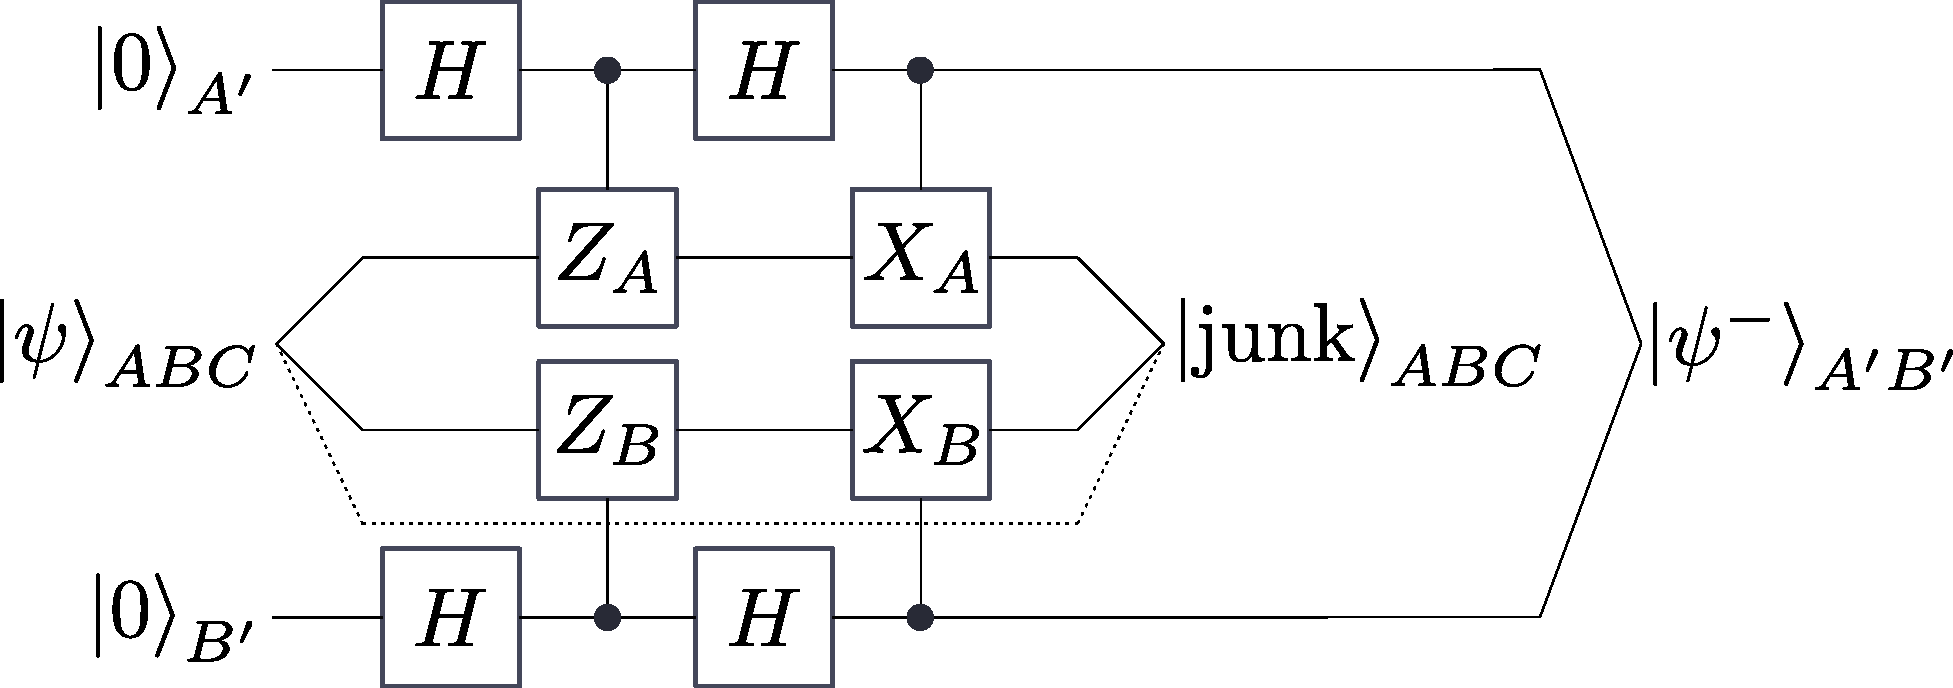
\includegraphics[width=0.95\textwidth]{chapters/selftesting/img/swap.pdf}
	\end{center}
	\caption{Circuit representation of the isometry $\Lambda$ extracting the target state, here $\ket{\psi^-}$, into ancillaries $A"B'$ with the correct dimesion. $H$ is the Hadamard gate, $Z$ and $X$ are control gates on the ancillaries.}
	\label{fig:swap}
\end{figure}

Let us first build the operators $X$ and $Z$ from Alice and Bob's observables, following
\begin{equation}
	\begin{split}
		Z_A = A_0, \qquad &X_A = A_1, \\
		Z_B = \frac{B_0 - B_1}{\sqrt{2}}, \qquad &X_B = \frac{B_0 + B_1}{\sqrt{2}}. \\ 
	\end{split}
\end{equation}
For $\Lambda$ to be a physical isometry, these operators have to be Hermitian and unitary.
Since we know that $A_x,B_y$ are Hermitian, and given that the sum of Hermitian matrices are Hermitian, our operators are Hermitian.
Trivially, $Z_A$ and $X_A$ are unitary. 
However, this is not the case for $Z_B$ and $X_B$, we need to \textit{regularise} them.
As detailed in \cite{Supic2019}, from an Hermitian operator $O$, we build an operator $O^\star$ by changing all the zero eigenvalues of $O$ to $1$, from which we construct a unitary operator $O'$ following $O'=|O^\star|^{-1} O^\star$.
Thanks to \refeq{aliceBobMeasEquivalence}, we can show that $Z_B'$ and $X_B'$ act the same way as $Z_B$ and $X_B$ on any state $\ket{\psi}$ following
\begin{equation}
	\begin{split}
		||(O_B' - O_B) \ket{\psi}|| &= ||(\id - O_B^\dag O_B)\psi|| \\
									&= ||(\id-|O_B|)\ket{\psi}|| \\
									&= ||(\id-|O_A O_B|)\ket{\psi}|| \\
									&\leq ||(\id-O_A O_B)\ket{\psi}|| \\
									&= 0
	\end{split}
\end{equation}
where $O$ can be replaced by either $X$ or $Z$.

We can now compute the effect of the isometry on the shared system and the ancillas
\begin{equation}
	\begin{split}
		\Lambda[\ket{00}_{A'B'} \otimes \ket{\psi}_{ABC}] = &\frac{1}{4}\Bigg[\ket{00}_{A'B'}\otimes(\id+Z_A)(\id+Z_B)\ket{\psi}_{ABC} \\
													   & + \ket{01}_{A'B'} \otimes X_B(\id+Z_A)(\id-Z_B)\ket{\psi}_{ABC} \\
													   & + \ket{10}_{A'B'} \otimes X_A(\id-Z_A)(\id+Z_B)\ket{\psi}_{ABC} \\
													   & + \ket{11}_{A'B'} \otimes X_AX_B(\id-Z_A)(\id-Z_B)\ket{\psi}_{ABC} \Bigg]
	\end{split}	
	\label{eq:swap_output}
\end{equation}
To simplify this, we first use \refeq{aliceBobMeasEquivalence} to derive the following equivalence relations
\begin{equation}
	X_A \ket{\psi} = X_B \ket{\psi}, \qquad Z_A \ket{\psi} = Z_B \ket{\psi}.
	\label{eq:ABMeasEquivalence}
\end{equation}
In \refeq{swap_output}, replacing $Z_A$ with $Z_B$ cancels all the term of the form $(\id\pm Z_A)(\id\mp Z_B)=(\id-Z_A^2)=0$, leading to
\begin{equation}
	\begin{split}
		\Lambda[\ket{00}_{A'B'} \otimes \ket{\psi}_{ABC}] = &\frac{1}{4}\Bigg[\ket{00}_{A'B'}\otimes(\id+Z_A)(\id+Z_B)\ket{\psi}_{ABC} \\
													   & + \ket{11}_{A'B'} \otimes X_AX_B(\id-Z_A)(\id-Z_B)\ket{\psi}_{ABC} \Bigg]
	\end{split}	
\end{equation}
By construction we have $\{Z_A,X_A\}=0$ and, from the anticommuting relation \refeq{anticommuting}, we have $\{Z_B,X_B\}\ket{\psi}=0$, which together with \refeq{ABMeasEquivalence} allow us to write
\begin{equation}
	\begin{split}
		X_A X_B (\id - Z_A)(\id-Z_B)\ket{\psi}_{ABC} &= (\id + Z_A)(\id +Z_B)X_A X_B \ket{\psi}_{ABC}\\
									 &= (\id + Z_A)(\id + Z_B)\ket{\psi}_{ABC} \\
									 &= (\id + Z_A)^2\ket{\psi}_{ABC} \\
									 &= 2(\id + Z_A)\ket{\psi}_{ABC}
	\end{split}
\end{equation}
Combing these expressions, the output of the isometry $\Lambda$ is given by
\begin{equation}
	\Lambda[ \id_{A'B'} \otimes \ket{\psi}_{ABC} ] = \underbrace{\frac{1}{2}\left( \ket{00}_{A'B'} + \ket{11}_{A'B'} \right)}_{\ket{\phi^+}_{A'B'}} \otimes \underbrace{\frac{1+Z_A}{2}\ket{\psi}_{ABC}}_{\ket{\text{junk}}_{ABC}}
	\label{eq:isometry}
\end{equation}

To get the self-testing statement ~\refeq{self-testing_statement}, Alice can apply an extra $\sigma_z$ gate on the $A'$ system, while Bob applies $\sigma_x$ on $B'$, transforming $\ket{\phi^+}_{A'B'}$ into $\ket{\psi^-}_{A'B'}$. These two gates can be freely embedded in $\Lambda$ as they are local unitaries on the ancillas.

Note that the purification space is left untouched under $\Lambda$. This can be seen from the construction of the operator $Z_A,X_A,Z_B$ and $X_B$, and they are composed of Alice and Bob observables, not acting on $\Hil^C$. 


\chapter{Robust self-testing of two-qubit maximally entangled state}

In the previous chapter, we examined the self-test of a two-qubit maximally entangled state from correlations achieving a maximal violation of the CHSH inequality.
However, such correlations can hardly be observed experimentally. 
Indeed, imperfect measurement calibrations as well as noisy and lossy quantum channels, creating and distributing the quantum state, will unavoidably lead to non-ideal correlations, i.e. not maximally violating the Bell inequality.
Furthermore, since any self-testing experiment can only collect a limited sample of Bell game rounds, the correlations are only estimated up to a certain confidence interval. 
Acknowledging such limitations, there is the need for self-testing protocols robust to the presence of imperfections in the correlations, also known as \textit{robust self-testing}.

There is multiple approaches to robust self-testing. 
Chronologically, the Mayers-Yao self-test was made robust in \cite{Magniez2006} while robust self-testing based on CHSH was introduced in \cite{Bardyn2009}.
A framework for the robust self-testing of the singlet was presented in \cite{McKague2012}.
Since then, numerous improvement were made to improve the robustness of self-testing, and to extended it to different scenario, e.g. multi-partite states or Bell scenarios with more inputs or outputs.

Here we present a method particularly relevant for the robust self-test of the singlet. 
This method is a numerical method based on Jordan's lemma and utilizing the CHSH inequality. 
Two notable methods than will not be discussed here are the analytical method based on operator inequalities presented in ~\cite{Kaniewski2016} and the numerical one SWAP method~\cite{Bancal2015}.
We then expose some fundamental limitations on robust self-testing based on the CHSH inequality.
Finally, we present a method that we developed, overcoming some of these limitations by extending robust self-testing of the singlet beyond the CHSH inequality.

\section{Extractability}

In robust self-testing, the goal is to use the correlation from a Bell game to bound the \textit{closeness} of the shared state, $\rho_{AB}$ to the target state $\psi_{AB}$.
Similarly to ideal-case self-testing, Alice and Bob can craft local isometries, $f_A$ and $f_B$, to extract the relevant degree of freedom from the shared state to reconstruct the target state.
Taking into account local isometries, a possible notion of \textit{closeness} is the so-called \textit{extractability} expressed as
\begin{equation}
	\Xi [\rho_{AB} \rightarrow \psi_{AB}] = \sup_{\{f_A,f_B\}} F((f_A \otimes f_B)[\rho_{AB}],\psi_{AB} \otimes \varrho_\text{junk})
	\label{eq:extractability_junk}
\end{equation}
where $F(\rho,\psi) = \left(\trr{\sqrt{\rho^{1/2}\psi\rho^{1/2}}}\right)^2$ is the square of the Uhlmann fidelity.

Isometry maping a state from one hilbert space $\Hil_1$ to another $\Hil_2$ can be thought of as a unitary operation on $\Hil_1 \otimes \Hil_2$ before discarding the $\Hil_1$ space.
This allows us to simplify the expression \refeq{extractability_junk} as
\begin{equation}
	\Xi [\rho_{AB} \rightarrow \psi_{AB}] = \sup_{\{\Lambda_A,\Lambda_B\}} F((\Lambda_A \otimes \Lambda_B)[\rho_{AB}],\psi_{AB}).
	\label{eq:extractability}
\end{equation}
A detailed proof of the equivalence of these two extractability definitions can be found in \cite{Sekatski2018}.


Note that the extractability is lower bounded by $1/2$ as it is always possible for Alice and Bob to construct isometries discarding the received state and preparing a new one with a fidelity of $1/2$ with respect to the target one. 
For example, if the target state is the singlet $\psi^{-}$, we can build isometries acting as
\begin{equation}	
	\left(\Lambda_A \otimes \Lambda_B\right)[\rho_{AB}] = \ket{1}\bra{1} \otimes \ket{0}\bra{0}.
\end{equation}
Therefore, a robust self-testing statement can be made if and only if $\Xi[\rho_{AB}]>1/2$.


\section{Robustness of CHSH-based singlet self-tests}

\subsection{Robust self-testing with two binary measurements}

As a device-independent protocol, no assumption are made on the dimension of the shared quantum state and the measurements.
However, in the particular case of a Bell game where Alice and Bob own two dichotomic measurements, i.e. with two outcomes, we can use Jordan's lemma to reduce the dimension of that game, to a game on $N$-qubits.
Indeed, Jordan's lemma states that for two Hermitian operators with eigenvalues $\pm1$ there exists a basis in which both operators are block-diagonal, with blocks of dimension $2 \times 2$.
To simplify further calculations, we consider these blocks to be in the $(\sigma_x,\sigma_z)$-plane.
This is done without loss of generality as Alice and Bob can always perform local rotations of their basis to recover that plane.
Alice and Bob observables can thus be written as a direct sum over these blocks 
\begin{equation}
	\begin{split}
	A_x = \bigoplus_i A_x^i &= \bigoplus_i \cos(\alpha_i)\sigma_h + (-1)^x \sin(\alpha_i)\sigma_m, \\
	B_y = \bigoplus_j B_y^j &= \bigoplus_j \cos(\beta_j)\sigma_z + (-1)^y \sin(\beta_j)\sigma_x,
	\end{split}
	\label{eq:block_observables}
\end{equation}
with $\sigma_{m,h} = (\sigma_z \pm \sigma_x)/\sqrt{2}$ and for some measurement angles $\alpha_i,\beta_j\in[0,\pi/2]$ for each block, indexed by $i$ and $j$.
Trivially, the CHSH operator defined in \refeq{CHSH_operator} inherits the same block structure and can be express following
\begin{equation}
	\mathcal{B}_\text{CHSH} = \bigoplus_{i,j} \mathcal{B}_\text{CHSH}^{i,j} = \bigoplus_{i,j} A_0^i \otimes (B_0^j + B_1^j) + A_1^i (B_0^j - B_1^j).
	\label{eq:block_operator}
\end{equation}

The shared quantum state $\rho_{AB}$ does not necessarily have a block diagonal structure. 
However, before measuring this state, Alice and Bob can always project it in their respective local basis to obtain the state
\begin{equation}
	\tilde{\rho}_{AB} = \bigoplus_{i,j} p(\alpha_i,\beta_j)\rho_{AB}^{i,j}
	\label{eq:}
\end{equation}
where $p(\alpha_i,\beta_j)$ is the success probability to project $\rho_{AB}$ in the $(i,j)$-block.
Note that the state $\tilde{\rho}_{AB}$ achieve the same CHSH violation as $\rho_{AB}$ thanks to the block structure of the CHSH operator
\begin{equation}
	S = \trr{\B_\text{CHSH}\rho_{AB}} = \sum_{i,j} p(\alpha_i,\beta_j) \trr{\mathcal{B}_\text{CHSH}^{i,j}\rho_{AB}^{i,j}}.
	\label{eq:}
\end{equation}

In the previous chapter, we have seen that in order to complete a self-testing statement we need to construct local isometries $\Lambda = \Lambda_A \otimes \Lambda_B$.
These local isometries can be constructed using the same block diagonal recipe 
\begin{equation}
		\Lambda = \bigoplus_{i,j} \Lambda_A^i \otimes \Lambda_B^j
	\label{eq:}
\end{equation}
with the isometry in each block acting as
\begin{equation}
	\Lambda_A^i: \mathcal{L}(\mathds{C}^2) \rightarrow \mathcal{L}(\mathds{C}^2), \qquad \Lambda_B^j: \mathcal{L}(\mathds{C}^2) \rightarrow \mathcal{L}(\mathds{C}^2).
	\label{eq:}
\end{equation}

From this block structure, the singlet extractability, i.e. \eqref{eq:extractability} with the singlet as the target state, is given by
\begin{equation}
	\Xi [\rho_{AB} \rightarrow \psi^{-}] = \sup_{\{\Lambda_A^i,\Lambda_B^j\}} \sum_{i,j} p(\alpha_i,\beta_j) F((\Lambda_A^i \otimes \Lambda_B^j)[\rho_{AB}^{ij}],\psi^{-}).
	\label{eq:block_extractability}
\end{equation}
Given that the probabilities $p(\alpha_i,\beta_j)$ are non-negative real numbers that sum up to $1$, by definition, the singlet extractability is given by a convex sum of the singlet extractability on two-qubit blocks.

\medbreak

To obtain a CHSH-based robust self-test of the singlet, we need to lower bound the singlet extractability with respect to all quantum realization achieving a given CHSH score $S$.
In order to do so, we can first obtain a lower bound on this extractability over all two-qubit blocks.
This can be done by first fixing the dependence of the isometries on the block indexes $(i,j)$.
Note that the resulting isomteries might not be maximize the singlet extractability, therefore, we will necessarily obtain a lower bound on \refeq{block_extractability}.
The minimum singlet fidelity over all two-qubit states and measurement choices compatible with a score $S$ is obtained by solving the optimisation
\begin{equation}
	\begin{split}
		O_{\min}(S)=\min_{i, j, \tau} \-\ & F(\Lambda_A^i \otimes\Lambda_B^j [\tau] ,\psi^-)\\
		\text{s.t.} \-\ &\trr{\matchal{B}_{CHSH}^{i,j}\, \tau} \geq S,\\
		& \tau \geq 0,\\
		& \tr{(\tau)} =1,\\
		& \tau^\dag = \tau.
	\end{split}
	\label{eq:sdp_extractability}
\end{equation}
The optimisation over all two-qubit states can be solved to arbitrary precision using semi-definite programming (see Appendix), while the optimisation over the blocks indexes is a non-linear optimisation over measurement angles.

Using the convex structure of \refeq{block_extractability}, it has been proven that the convex roof of $O_{\min}(S)$ over all CHSH scores, $f(S)$ gives a lower bound on the singlet-extractability with respect to the CHSH score~\cite{Sekatski2018}.
Therefore, from a CHSH score $S$, one can hope to extract a singlet fidelity of at most 
\begin{equation}
	\mathcal{F}(S)=\max\left(1/2, f(S)\right).
	\label{eq:}
\end{equation}

\subsection{Robustness bounds}

To asses the performance of robust self-testing, we are interested in the evolution of the extractability with respect to the Bell violation.
In particular, the minimum violation for which a non-trivial fidelity to the target state can be extracted is called the \textit{robustness bound}.
This bound is crucial as any implementation of a self-testing protocol is required to have the capabilities to achieve a Bell violation at least as high as the robustness bound.

To glean the robustness bound with the method presented in the previous section, we first need to choose the local isometries $\Lambda_A^i$ and $\Lambda_B^i$ appearing in \refeq{sdp_extractability}.
These isometries are completely-positive trace preserving maps acting on qubit space and parametrised by Alice and Bob measurement choice, respectively.
A relevant pick for such maps has been reported in \cite{Kaniewski2016}.
For the block $i$, let Alice's map be a dephasing map of the form
\begin{equation}
	\Lambda_A^i(\alpha_i)[\rho_{AB}] = \left( \frac{1+g(\alpha_i)}{2}\id\rho_{AB}\id+\frac{1-g(\alpha)}{2}\Gamma(\alpha_i)\rho_{AB}\,\Gamma(\alpha_i)\right),
	\label{eq:dephasing_maps}
\end{equation}
with a dephasing strength
\begin{equation}
	g(\alpha_i)=(1+\sqrt{2})(\cos{\alpha_i}+\sin{\alpha_i}-1)
	\label{eq:dephasing_strength}
\end{equation}
and a dephasing direction
\begin{equation}
	\Gamma(\alpha_i) = \begin{cases}
      \sigma_h, & \text{if}\ \alpha_i\leq\frac{\pi}{4} \\
      \sigma_m, & \text{otherwise}.
    \end{cases}
	\label{eq:dephasing_direction_alice}
\end{equation}
For the block $j$ and the corresponding measurement angle $\beta_j$, Bob's map is of the same form, but with a dephasing direction given by
\begin{equation}
	\Gamma(\beta_j) = \begin{cases}
      \sigma_h, & \text{if}\ \beta_j\leq\frac{\pi}{4} \\
      \sigma_m, & \text{otherwise}.
    \end{cases}
	\label{eq:dephasing_direction_bob}
\end{equation}

We can now solve the optimisation \refeq{sdp_extractability} and, from the convex roof, obtain $\mathcal{F}(S)$, the lower bound on the singlet extractability as a function of the CHSH score.
This function is depicted in \reffig{fidCHSH}.
A non-trivial fidelity is achieved for any CHSH violation greater than $S \approx 2.11$, the robustness bound. 

It is worth noting that, using an analytical approach~\cite{Kaniewski2016}, this bound has been found at $S=(16+14\sqrt{2})/17\approx2.11$, compatible with the numerical result we present here.

\begin{figure}
	\begin{center}
		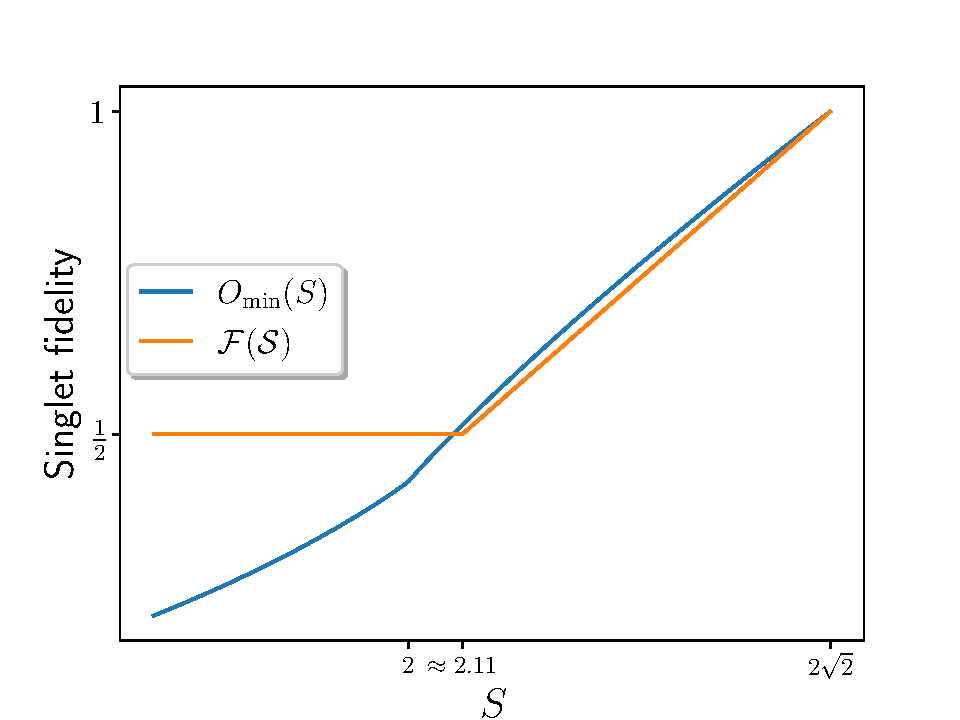
\includegraphics[width=0.95\textwidth]{chapters/selftesting/img/fidCHSH.pdf}
	\end{center}
	\caption{Singlet fidelity with respect to CHSH.}
	\label{fig:fidCHSH}
\end{figure}

\subsection{Limits of CHSH-based singlet self-testing}

While continuous efforts are made to improve the robustness bound of CHSH-based self-testing, another approach focuses on finding the \textit{threshold CHSH score} below which no self-testing statement can be made.
Surprisingly, it has been demonstrated~\cite{Coopmans19} that this threshold does not coincide with the local bound $S=2$.
The demonstration is based on an example of a state that achieve a violation of the CHSH inequality with a score of $S=2.0014$ while having a singlet extractability of $1/2$.

\medbreak

This proof raised numerous questions. 
First, as photonic implementations seems more desirable for technological applications of self-testing, most photonic loop-hole free Bell test realisation are based on polarization entangled photons for which detection efficiencies of $\approx 90\%$ are required to achieve a score higher that $2.11$~\cite{Vivoli2015b}. 
Such detection efficiencies are beyond the realm of current possibilities. 
Therefore, if the threshold CHSH score is close to $2.11$, self-testing the singlet will be extremely challenging.
Secondly, if that threshold is close to the local bound, efforts need to be put to craft better local isometries than the one proposed in \cite{Kaniewski2016}.
Thirdly, and more fundamentally, it raises the question of the type of resources needed for self-testing.
The CHSH threshold prove that under local operation (LO) only, singlet-extraction is not possible from any CHSH violation.
However, if Alice and Bob can share classical information (LOCC), a singlet state can always be extracted from the slightest CHSH violation~\cite{Bardyn2009}. 
Therefore, it would be interesting to explore if this threshold still occurs under other regimes such as local operations and shared randomness (LOSR).
Finally, it is worth exploring whether this threshold appears when the singlet-fidelity in the extractability is replaced by another quantity such as the trace distance. 

\medbreak

In an attempt to answer some of these question, in Article 1~\cite{Valcarce2020} we search for the maximum CHSH score resulting in a trivial singlet extractability
\begin{equation}
	\begin{split}
		\sup_{\rho_{AB}}\ &\sum_{i,j} p(\alpha_i,\beta_j) \tr (\mathcal{B}_\text{CHSH}^{i,j} \rho_{AB}^{i,j})\\
\textnormal{s.t.}\ &\,\Xi[\rho_{AB}\rightarrow \psi^-] \leq \frac{1}{2}.
	\end{split}
	\label{eq:CHSH_threshold}
\end{equation}
As the proof can be constructive, we chose to limit ourselves to a subset of this optimisation problem, considering 3 two-qubit blocks for each party, from which we derived a family of measurement and states.
More specifically, the states we consider are a mixture between separable states and the singlet state.
Then, from the parametrisation of extremal single-qubit CPTP maps~\cite{Verstraete2002}, we derived a relaxation of the effect of all single-qubit maps on our state, simplifying greatly the problem \refeq{CHSH_threshold}.
Indeed, for any state of the family we consider, the singlet extractability can thus be expressed as a non-linear optimisation of a Lipschitz continuous function, which can be numerically bounded~\footnote{We developed an algorithm to obtain such a bound, see https://gitlab.com/plut0n/bcert}.
When optimising the relaxed version of \refeq{CHSH_threshold} over the family of state we specified, we discovered a state yielding a CHSH score of $\approx 2.05$ while maintaining a trivial singlet-extractability, pushing the CHSH threshold by an order of magnitude.

Importantly, our result show the limitation of CHSH-based self-testing as the \textit{CHSH threshold} lays in the $[2.05,2.11]$ range.


\section{Robust singlet self-testing beyond CHSH}

In an attempt to make robust self-testing more accessible to experimental implementations as well as technological applications, there is the need for protocols lowering the requirement on detection efficiencies and noise limitations.
In the previous section, we saw that robust CHSH-based self-testing has been only proven for violation of $S\approx 2.11$ and can not be made for violation below $2.05$.
These relatively high CHSH score are hardly in reach experimentally, and, as such, only one self-testing experiment as been reported to date~\cite{Bancal2021}.

It is in this scope that in Article 2 we proposed a new protocol for robust self-testing.
Our approach is based on a more refined analysis of the correlations which are needed to compute the CHSH score, i.e. our protocol does not require any additional data.
Instead of using a single Bell inequality, our protocol relies on a family of Bell inequalities, \textit{generalized CHSH inequalities}
\begin{equation}
S_\theta = \sqrt{2}(\cos(\theta) \underbrace{\mean{A_0(B_0+B_1)}}_{X} + \sin(\theta)\underbrace{\mean{A_1(B_0-B_1)}}_{Y})
	\label{eq:}
\end{equation}
parametrized by an angle $\theta \in [0,\pi/2]$, for which we derived robust self-testing statements.

As our approach applies to a Bell game with two dichotomic measurements, we proved self-testing statement utilizing Jordan's lemma, following the steps explained in the previous section. 
Analogously to the CHSH-case, we obtained the robstuness bound by minimizing the singlet fidelity over all state and measurement choices, for fixed isometries.
We crafted isometries with a dependency in both the local measurement choice and $\theta$.
More specifically, these isometries are inspired by the one presented in \refeq{dephasing_maps}, with a couple of tweaks, notably a dephasing strength depending on $\theta$, and for one party, an aditional rotation along $\sigma_y$ as well as a dephasing direction depending on the angle of measurement and $\theta$.

We then provide a robust self-testing statement recipe for any given correlator pair $(X,Y)$.
From a list of parameters $\theta$ and the corresponding robustness bound $S_\theta^\text{bound}$ that we provide, one can hope to obtain a singlet-extractability of 
\begin{equation}
	\max_\theta \mathcal{F}(S_\theta) = \max_\theta \left[ \begin{cases}
			\frac{1}{2},& \text{if} S_\theta \leq S_\theta^\text{bound}, \\
			\frac{1}{2}\left(1+\frac{S_\theta - S_\theta^\text{bound}}{2\sqrt{2}-S_\theta^\text{bound}}\right), & \text{otherwise}.
	\end{cases} \right]
	\label{eq:singlet-extractability-theta}
\end{equation}
The maximum singlet-extractability over all $\theta$, as a function of correlator pairs $(X,Y)$ is depicted in \reffig{generalizedCHSHfid}.

Comparing to CHSH-based self-testing, our protocol achieve higher singlet-extractability for any correlator $X\neq Y$.
Furthermore, our protocol can be used to perform self-tests for correlation leading to CHSH violation below the robustness bound of $S\approx 2.11$, below which no self-testing statement has been proven, and even below the currently known CHSH threshold of $2.05$, providing enough imbalance between the correlators, e.g. $X \gg Y$.
Therefore, this protocol makes self-testing implementations more accessible, especially in a case of imbalanced correlator relevant for ?

\begin{figure}
	\begin{center}
		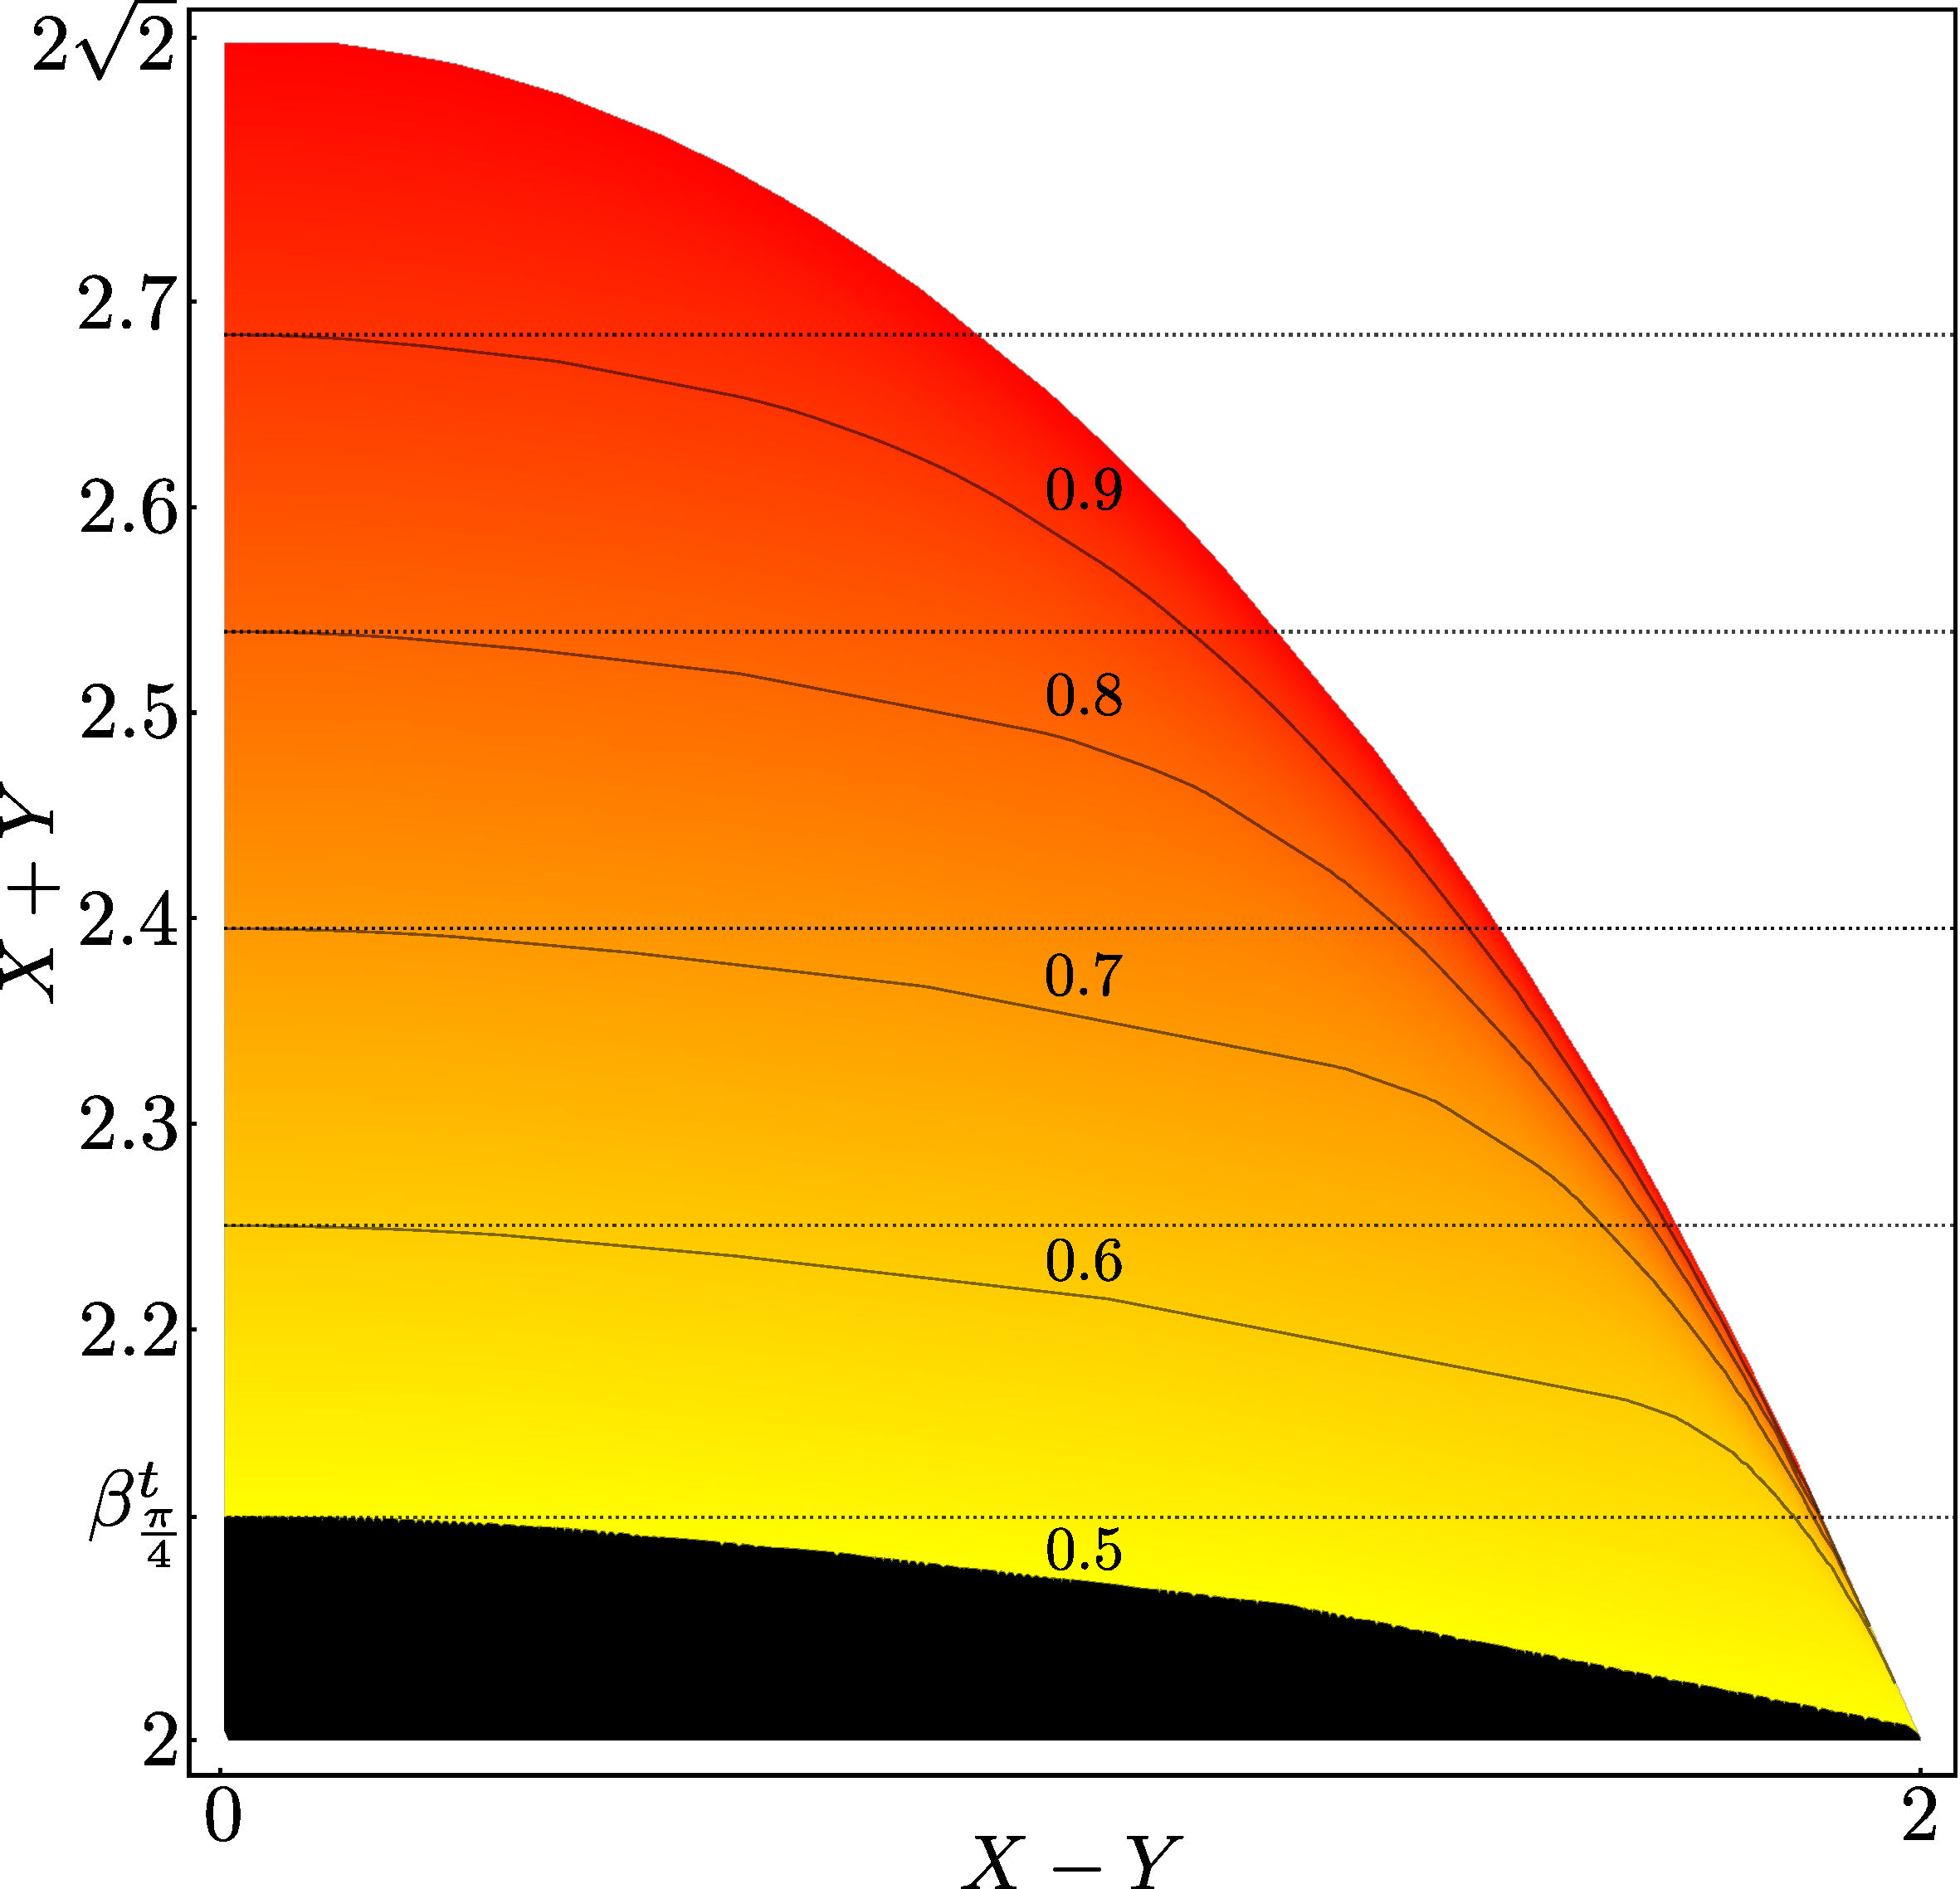
\includegraphics[width=0.95\textwidth]{chapters/selftesting/img/generalizedCHSH.pdf}
	\end{center}
	\caption{Solution to \refeq{singlet-extractability-theta} for all pair of correlator $(X,Y)$. The dashed lines represent different singlet-extractabilities using CHSH, while the solid line shows the singlet-extractability achieved using the most fitting generalized CHSH inequality. Correlators in the black zone can not be used to make self-testing statement with our method.}
	\label{fig:generalizedCHSHfid}
\end{figure}



\titleformat{\article}
   {\normalfont\Large\bfseries}{\thearticle}{1em}{}

\chapter*{Article 1}
\label{article_minCHSH}
\article{What is the minimum CHSH score certifying that a state resembles the singlet?}

\begin{center}
\textrm{\LARGE What is the minimum CHSH score certifying that a state resembles the singlet?}

\vspace{2cm}

\normalsize
Xavier Valcarce$^1$, Pavel Sekatski$^1$, Davide Orsucci$^1$, Enky Oudot$^{1,2}$, Jean-Daniel Bancal$^{1,2}$, and Nicolas Sangouard$^1$
\bigbreak

{\footnotesize
$^1$ Departement Physik, Universität Basel, Klingelbergstraße 82, 4056 Basel, Schweiz \\
$^2$ Département de Physique Appliquée, Université de Genève, 1211 Genève, Suisse
}

\raggedright
\bigbreak
\faLink \quad \href{https://quantum-journal.org/papers/q-2020-03-23-246/}{Quantum, volume 4, page 246} \\
\faLink \quad \href{https://arxiv.org/abs/1910.04606}{arXiv preprint: 1910.04606}
\vspace{1cm}

\centering
\textbf{Abstract}
\bigbreak

A quantum state can be characterized from the violation of a Bell inequality.
The well-known CHSH inequality for example can be used to quantify the fidelity (up to local isometries) of the measured state with respect to the singlet state.
In this work, we look for the minimum CHSH violation leading to a non-trivial fidelity.
In particular, we provide a new analytical approach to explore this problem in a device-independent framework, where the fidelity bound holds without assumption about the internal working of devices used in the CHSH test.
We give an example which pushes the minimum CHSH threshold from $\approx 2.0014$ to $\approx 2.05$, far from the local bound.
This is in sharp contrast with the device-dependent (two-qubit) case, where entanglement is one-to-one related to a non-trivial singlet fidelity.
We discuss this result in a broad context including device-dependent/independent state characterizations with various classical resources.

\end{center}

\chapter*{Article 2}
\article{Self-testing two-qubit maximally entangled states from generalized Clauser-Horne-Shimony-Holt tests}

\centering
\textrm{\LARGE Self-testing two-qubit maximally entangled states from generalized Clauser-Horne-Shimony-Holt tests}

\vspace{2cm}

\normalsize
Xavier Valcarce$^1,2$, Julian Zivy$^1,2$, Nicolas Sangouard$^1,2$, and Pavel Sekatski$^2$
\bigbreak

{\footnotesize
	$^1$ Université Paris-Saclay, CEA, CNRS, Institut de Physique Théorique, 91191 Gif-sur-Yvette, France \\
	$^2$ Departement Physik, Universität Basel, Klingelbergstraße 82, 4056 Basel, Schweiz
}

\raggedright
\bigbreak
\faLink \quad \href{https://journals.aps.org/prresearch/abstract/10.1103/PhysRevResearch.4.013049}{Phys. Rev. Research 4, 013049} \\
\faLink \quad \href{https://arxiv.org/abs/2011.03047}{arXiv preprint: 2011.03047}
\vspace{1cm}

\centering
\textbf{Abstract}
\bigbreak

Device-independent certification, also known as self-testing, aims at guaranteeing the proper functioning of untrusted and uncharacterized devices.
For example, the quality of an unknown source expected to produce two-qubit maximally entangled states can be evaluated in a bi-partite scenario, each party using two binary measurements.
The most robust approach consists in deducing the fidelity of produced states with respect to a two-qubit maximally entangled state from the violation of the CHSH inequality.
In this paper, we show how the self-testing of two-qubit maximally entangled states is improved by a refined analysis of measurement statistics.
The use of suitably chosen Bell tests, depending on the observed correlations, allows one to conclude higher fidelities than ones previously known.
In particular, nontrivial self-testing statements can be obtained from correlations that cannot be exploited by a CHSH-based self-testing strategy.
Our results not only provide novel insight into the set of quantum correlations suited for self-testing, but also facilitate the experimental implementations of device-independent certifications.


\part{Device-independent communication and cryptography}

\chapter{Overview on device-independent key distribution}

\section{From Bell inequality to security}

\section{A DIQKD protocol}

\section{Security definition}


\chapter{Entropy bounds}
\label{chap:entropybound}

\section{Key rate}

To asses the performance of DIQKD protocols we need to compute the \textit{key rate}, labelled $r$, corresponding to the amount of key bit that can be extracted per round.
These extracted key bits are secret, i.e. provably unknown to Eve, and correct, i.e. identical for Alice and Bob.
Therefore, key rates can be derived to take into account specific attacks implemented by Eve, and specific error-correction protocol.
In the following, we discuss key rates that were first derived with the assumption that quantum devices are independent and identically distributed (IID) over the rounds of the protocols, i.e. that the devices are memoryless, measurements $\hat{A}_x,\hat{B}_y$ are the same through the protocol and the distributed state for $n$-round is of the form $\ket{\psi}_{ABE}^{\otimes n}$.
This assumption limits Eve's range of attack to what is known as collective attack.
However, using the \textit{entropy accumulation theorem}~\cite{Dupuis2019,Dupuis2020}, it has been shown that the key rates we present here hold under general attacks, dropping the need for the IID assumption~\cite{ArnonFriedman2019}.

\medbreak

Intuitively, the key rate is given by the mutual information between the outcomes of the generation rounds, $A_0$ and $B_2$, used to generate the key (correctness) and is limited by the amount of information Eve has on $A_0$ (secrecy).
In the asymptotic limit of an infinite amount of round, where one-way error correction is used and where the correlations $p(ab|xy)$ can be computed exactly, the key rate is lower-bounded by the Devetak-Winter bound~\cite{Devetak2005}
\begin{equation}
	r \geq r_\mathrm{DW} = I(A_0 : B_2) - \chi(A_0 : E)
	\label{eq:Devetak-Winter}
\end{equation}
where $I$ is the mutual information, $\chi$ corresponds to the Holevo bound and $E$ denotes the quantum-side information Eve stored during the protocol.
Note that the key rate can be expressed using conditional von Neumann entropies $H(\centerdot|\centerdot)$ following
\begin{equation}
	\begin{split}
		r_\mathrm{DW} &= I(A_0 : B_2) - \chi(A_0 : E) \\
					  &= H(A_0)-H(A_0|B_2) - (H(A_0)- H(A_0|E)) \\
					  &= H(A_0|E) - H(A_0 | B_2).
	\end{split}
\end{equation}

The remaining challenge is to bound these two term, and in particular to upper-bound the Holevo quantity directly from the correlations $p(ab|xy)$, as no assumption can be made on Eve's system and the quantum devices. 
In the following two sections we will described two methods to tackle this bound, the first one utilizing the CHSH score, the second one based on a more refined analysis of the correlations.

\section{CHSH-based security}

\subsection{Key rate from the CHSH score}
\label{sec:pironio}

In \cite{Pironio2009}, the first upper-bound on the Devetak-Winter bound has been derived.

This approach makes use of an additional symmetrisation step in the protocol presented in the previous chapter.
The symmetrisation step allow Alice and Bob to obtain uniform marginals.
In order to do so, Alice and Bob can simply XOR their key bits with a public random string that is shared over the classical channel.

Thanks to the symmetrisation step, the mutual information between Alice and Bob's raw key simply reads
\begin{equation}
	I(A_0 : B_2) = H(A_0) - H(A_0|B_2) = 1 - h(Q)
	\label{eq:}
\end{equation}
where $Q=p(a=b|xy)-p(a\neq b |xy)$ is the quantum error bit rate (Qber) and $h$ is the binary entropy $h(x)=-x \log_2(x) - (1-x)log_2(1-x)$.

From the parameter estimation step of the protocol presented above, Bob can compute the CHSH score $S=\mean{\hat{A}_0 \hat{B}_0} + \mean{\hat{A}_0 \hat{B}_1} + \mean{\hat{A}_1 \hat{B}_0} - \mean{\hat{A}_1 \hat{B}_1}$.
From this score and using Jordan's lemma, an upper-bound on the Holevo quantity appearing in \refeq{Devetak-Winter} is derived
\begin{equation}
	\chi(A_0 : E) \leq h\left(\frac{1+\sqrt{(S/2)^2-1}}{2} \right).
	\label{eq:holevo_pironio}
\end{equation}

Finally, from this two results, a lower bound on the DIQKD key rate is given by
\begin{equation}
	r \geq r_\mathrm{P} = 1 - h\left(\frac{1+\sqrt{(S/2)^2-1}}{2} \right) - h(Q).
	\label{eq:pironio}
\end{equation}

\subsection{Coarse grained error-correction}

When presenting the protocol in the previous chapter, we assumed that Alice and Bob have binary measurements with outcomes $\pm 1$.
A more general approach would allow both parties to have measurements with more outcomes, that could ultimately be binned to form the raw key.
Non-binary outcomes naturally occur in the presence of loss, as loss might lead to no measurement outcomes, which can be accounted as an extra outcome.
Interstingly, Bob can use the extra information of the non-binned or \textit{coarse} outcomes of $B_2$ to reduce the cost of error-correction~\cite{Ma2012}.
This \textit{coarse grained error correction} is given by
\begin{equation}
	\begin{split}
		I(A_0 : B_2) &= 1-H(A_0|B_2) \\
					 &= 1-H(A_0,B_2) - H(B_2) \\
					 &= 1-\sum_b \left( \sum_{a = \pm1} -p(ab|02)\log_2(p(ab|02)) \right) \\
					 &\qquad - p(b|02)\log_2(p(b|02)).
	\end{split}
	\label{eq:Ma}
\end{equation}
Note that this error-correction trivially reduces to $1-h(Q)$ in case Bob has only two outcomes.

Therefore, a tighter lower-bound on the key rate is
\begin{equation}
	r \geq r_\mathrm{ML} = 1 - h\left(\frac{1+\sqrt{(S/2)^2-1}}{2} \right) - H(A_0|B_2).
	\label{eq:Makr}
\end{equation}


\subsection{Noisy Preprocessing}

In the case of device-dependent QKD~\cite{Renner2005,Kraus2005,Renes2007}, it has been shown that Eve's uncertainty might increase if Alice includes a \textit{noisy-preprocessing} step following the measurement step of the DIQKD protocol we consider here~\cite{Ho2020}.
This is done by introducing a trusted source of noise on the measurement Alice uses for key generation rounds, which acts as a bit-flip operation on the binned outcome of $\hat{A}_0$ occurring with a probability $q$, fixed by Alice.
Formally, this is the transformation
\begin{equation}
	p(a|0y) \rightarrow (1-q)\,p(a|0y) + q\, p(-a|0y).
\end{equation}
We denote $A_0'$ the raw key bit of Alice after noisy pre-processing.

For a CHSH score $S$ and a noisy preprocessing probabliy $q$, the Holevo quantity is upper bounded by
\begin{equation}
	\begin{split}
		\chi(A_0' : E) \leq I_q(S) = &h\left(\frac{1+\sqrt{(S/2)^2-1}}{2}\right) \\
									&-h\left(\frac{1+\sqrt{1-q(q-1)(8-S^2)}}{2} \right),
	\end{split}	
\end{equation}
which is equivalent to \refeq{holevo_pironio} when $q=0$, and smaller otherwise.

Combined with the coarse grained error-correction term \refeq{Ma}, we obtain the following lower bound on the key rate
\begin{equation}
	r \geq r_\mathrm{Ho} = 1 - I_p(S) - H(A_0'|B_2).
	\label{eq:Ho}
\end{equation}


\subsection{Robustness of CHSH-based security}
\label{sec:robust_DIQKD}

To grasp the requirements for experimental implementations of DIQKD, we need to study the behaviour of the key rate for some specific quantum model and losses.

\medbreak

Intuitively, it is worth exploring the behaviour of the key rate when the source sends a singlet state $\ket{\psi}=\frac{1}{\sqrt{2}}(\ket{00}+\ket{11})$, as this state saturate the CHSH inequality and thus should yield a key rate of $1$ in the absence of losses.

We consider measurements to be as general as possible on the $(\sigma_x-\sigma_z)$-plane. This is, measurements characterized by the POVMs associated with outcomes $\{+1,-1\}$
\begin{equation}
	\begin{split}
		\hat{A}_x\,:\, \{M(\alpha_x),\, \id-M(\alpha_x)\} \\
		\hat{B}_y\,:\, \{M(\beta_y),\, \id-M(\beta_y)\}
	\end{split}	
\end{equation}
with $M(\theta) = \frac{1}{2}\left(\id + \cos(\theta)\sigma_z + \sin(\theta)\sigma_x \right)$ and the angles $\alpha_x,\beta_y\in[0,\pi/2]$.
To verify our intuition in the absence of loss, without noisy preprocessing $q=0$, and with the optimal angles $(\alpha_0,\alpha_1)=(0,\pi/2)$ and $(\beta_0,\beta_1,\beta_2)=(\pi/4,-\pi/4,0)$, we indeed obtain a key rate of
\begin{equation}
	r \geq 1-h\left(\frac{1+\sqrt{(S/2)^2-1}}{2}\right)-h(Q) = 1 - h(1) - h(1) = 1.
\end{equation}

In the presence of loss, we need to address the possibility of the shared state being lost before the measurement, which would result in the absence of outcome.
We label $\eta\in[0,1]$ the efficiency of the quantum devices, i.e. the shared state is lost with probability $1-\eta$.
If the state is lost, Alice and Bob can recover binary outcomes by binning the no-outcome event as $+1$.
Thus, their POVMs becomes
\begin{equation}
	\{M^{+1},\,M^{-1}\} \rightarrow \{\eta M^{+1}+(1-\eta) \id,\, 1-\left(\eta M^{+1}+(1-\eta) \id\right)\}.
\end{equation}
However for his measurement $B_2$, Bob can simply consider all three outcomes, with the corresponding POVM
\begin{equation}
	B_2\, : \, \{\eta M(\beta_2),\, \eta (1-M(\beta_2)),\, (1-\eta) \id \},
\end{equation}
since exploiting coarse grained outcomes can reduce the cost of error-correction when using \refeq{Ma}.

To study the robustness of CHSH-based key rates, we optimise the different key rates \refeq{pironio}, \refeq{Makr} and \refeq{Ho}, over all measurement angles $\alpha_x,\beta_y$, for a decreasing efficiency $\eta$. 
When considering noisy preprocessing, we also optimize the key rate over the parameter $q$ of \refeq{Ho}.
These key rates are shown by the blue curves in figure Fig.. 
Most interestingly, using noisy preprocessing and coarse grained error-correction, we obtain a critical efficiency of $\eta \approx 0.903$, below which no key can be extracted.

For a more general approach, we study the robustness of the CHSH-based key rates for all partially entangled pure two-qubit states of the form
\begin{equation}
	\ket{\psi}_\theta = \frac{1}{2}\left(\cos(\theta)\ket{00}+\sin(\theta)\ket{11}\right)
\end{equation}
with $\theta\in[0,\pi]$.
This is done by adding the parameter $\theta$ as an optimisation parameters when optimising for the key rate.
The results are given by the orange curves in Fig.
Thee key rate is more tolerant to loss for these states, as the critical detection efficiency drop to $\eta\approx 0.826$.

\section{DIQKD security proof beyond CHSH}

In the previous section, we presented how provably secure key bits can be extracted from the CHSH score.
If improvement on the key rate has been made by including coarse grained error-correction and noisy preprocessing, the security proof is still fundamentally limited by the CHSH score.
To improve the resistance to losses, a natural approach is to derive a security statement from a more refined analysis of the observed statistics $\{p(ab|xy)\}$.
Conveniently, since the CHSH score is computed from these correlations, no extra steps or assumptions on the DIQKD protocol are required. 

\subsection{Security statement from generalized-CHSH score}
\label{sec:Pavel}

Generalized CHSH score $S_\theta=\sqrt{2}(\cos(\theta)X+\sin(\theta)Y)$, obtain from the genrealized CHSH operator $\mathcal{B}_\theta$, allow to exploit the knowledge of the correlator pair
\begin{equation}
	\begin{split}
		X = \mean{A_0 \otimes (B_0+B_1)},\\
		Y = \mean{A_1 \otimes (B_0-B_1)}.
	\end{split}
\end{equation}
We have seen in the previous part that generalized CHSH inequalities, compared to CHSH, can be advantageous for a device-independent protocol that is self-testing~\cite{Valcarce2022}.
Intuitively, these inequalities can be useful for DIQKD as well.
The intuition comes from the correlator pair $X,Y$ allowing to differentiate between the contributions of measurements $\hat{A}_0$, used for key generation, and $\hat{A}_1$ solely used to test the quantum devices.
From this extra degree of freedom, $\hat{A}_0$ can be designed to be more correlated with $\hat{B}_2$, reducing the cost for error-correction while maintaining a constant bound on Eve's entropy on the key, e.g. by reducing the contribution of the correlator $X$ in the security proof.

In Article 3, we investigate this intuition, paving the way for DIQKD security proofs beyond the CHSH score. 
We here provide a sketch of the proof, for more detail please refer to \cite{Sekatski2021} or, alternatively, to \cite{Woodhead2021}.


\medbreak

Binning the outcomes $A_x,B_y$ for $x,y\in\{0,1\}$, allow to utilize Jordan's lemma to express Alice and Bob observables as block diagonal operators on qubits
\begin{equation}
	\begin{split}
		\hat{A}_x = \bigoplus_i \hat{A}_x^i &= \bigoplus_i \mathbf{\alpha_x^i} \begin{pmatrix}\sigma_z \\ \sigma_x\end{pmatrix}, \\
		\hat{B}_y = \bigoplus_j \hat{B}_y^j &= \bigoplus_j \mathbf{\beta_y^i} \begin{pmatrix}\sigma_z \\ \sigma_x\end{pmatrix},
	\end{split}
\end{equation}
with unit vectors $\mathbf{\alpha_x^i} = (\alpha_x^{i,0},\alpha_x^{i,1})$ and $\mathbf{\beta_y^j} = (\beta_y^{j,0},\beta_y^{j,1})$.
Without loss of generality we can also write the shared state as
\begin{equation}
	\ket{\psi}_{ABE} = \bigoplus_{i,j} \sqrt{p_{i,j}} \ket{\psi}_{ABE}^{i,j}	
	\label{eq:}
\end{equation}
with $\ket{\psi}_{ABE}^{i,j} \in \mathds{C}^2_A \otimes \mathds{C}^2_B \otimes \Hil_E^{(4)}$ and for some probability distribution $p_{i,j}$.
This allow to express Eve's uncertainty on the key, after noisy preprocessing, as the convex sum
\begin{equation}
	H(A_0'| E) = \sum_{i,j} p_{i,j} H_{i,j}(A_0' | E)
	\label{eq:H_convex}
\end{equation}
where $H_{ij}(A_0' | E)$ is computed from the state $\ket{\psi}_{ABE}^{i,j}$.
To lower bound that quantity, we can minimize the entropy $H_{ij}(A_0 | E)$ over all four-qubits quantum model compatible with a generalized CHSH score $S_\theta$.
If the minimization gives a convex function of $S_\theta$, from \refeq{H_convex}, that function acts as a lower bound on Eve's entropy. 
If that is not the case, an extra convexification step can be added before obtaining the lower bound~\cite{Sekatski2021}.

To simplify the minimization problem, we include a symmetrisation step, as explained in Sec~\ref{sec:pironio}, such that Alice and Bob have uniform marginals.
Since no such marginals appear in the constraint of the minimization problem, the symmetrisation step allow to consider a minimization over only Bell diagonal states~\cite{Pironio2009}
\begin{equation}
	\ket{\psi}_{ABE}^{i,j} = \sum_k \sqrt{L_k^{i,j}} \ket{\phi_k} \otimes \ket{i}_E
	\label{eq:psi_ABE_reduced}
\end{equation}
where $\ket{\phi_k}=\{\ket{\phi^+},\ket{\phi^-},\ket{\psi^+},\ket{\psi^-}\}$ are the Bell states defined in \refeq{bell_states} and $L_k$ are  eigenvalues we collect in a vector $\mathbf{L}=(L_1,L_2,L_3,L_4)$.

The objective of the minimization, Eve's entropy, reads
\begin{equation}
	H(A_0'|E)_{i,j} = H(A_0') - H_{i,j}(\rho_E) + \sum_{a' = \pm 1} p(a'|x=0)H_{i,j}(\rho_{E|a'})	
	\label{eq:}
\end{equation}
where $\rho_E$ is Eve's subsystem and $\rho_{E|a'}$ is Eve's subsystem conditioned on the key bit $a' = (1-q)\,a + q\,(-a)$ occurring with probability $p(a')$, for a noisy preprocessing bit flip probability of $q$.
This expression can be simplified as $H(A_0')=1$ from the symmetrisation step.
Furthermore, we have $H_{i,j}(\rho_E)=H_{i,j}(\mathbf{L})$ and $H_{i,j}(\rho_{E|a'})$ can be express as a function $f_{i,j}(\mathbf{L},\alpha_0^i)$ of the eigenvalues $\mathbf{L}$ and Alice's measurement angle $\mathbf{\alpha_0^i}$.

Finally, we can solve the minimization problem 
\begin{equation}
	\begin{split}
		\min_{L,\alpha_0^i,\alpha_1^i,\beta_0^j,\beta_1^j} &1 - H_{i,j}(\mathbf{L}) + f_{i,j}(\mathbf{L},\alpha_0^i) \\
		&\mathrm{s.t.}\quad 
		\mathcal{B}_\theta (\mathbf{L},\alpha_0^i,\alpha_1^i,\beta_0^j,\beta_1^j) \geq S_\theta
	\end{split}
	\label{eq:}
\end{equation}
where $\mathcal{B}_\theta (\mathbf{L},\alpha_0^i,\alpha_1^i,\beta_0^j,\beta_1^j)$ is the generalized CHSH operator on two-qubits, parametrized by $\theta$, for Alice and Bob's measurement angles $(\alpha_0,\alpha_1,\beta_0,\beta_1)$, applied on states of the form \refeq{psi_ABE_reduced} characterized by $\mathbf{L}$.

In Article 3, we solve that minimization for all $\theta$. This gave us the bound on the conditional entropy $1-I_{\theta,q}(X,Y)\leq H(A_0|E)$ and, hence, the lower bound on the key rate
\begin{equation}
	r \geq r_\mathrm{Sek} = 1 - I_{\theta,q}(X,Y) - H(A_0'|B_2).
	\label{eq:Sekatstki}
\end{equation}
Interestingly, this approach achieves higher key rate than CHSH-based key rates, except when correlators satisfies $X(X+Y)=4$ for which obtained key rates are equal.
When considering optimal noisy preprocessing, the gap in improved key rate diminish but is still non-neglectible.
Applied to the concrete case of a singlet state as explained in \ref{sec:robust_DIQKD}, the criticial detection efficiency drops from $\approx 0.903$ to $\approx 0.900$ when using generalized CHSH security proof.
However, for partially entangled two-qubit states, there is no improvement in critical detection efficiency.
Note that in \cite{Woodhead2021}, a DIQKD security proof from the generalized CHSH score has been derived analyticaly. The reported advantages in key rate and critical efficiencies are indentical to the ones found using our proof.

\medbreak


\subsection{Security statement from all correlations}
\label{sec:Brown}

In \cite{Brown2021} a deviceindependent lower bound on von Neumann entropies has been derived based on all the correlations $\{p(ab|xy)\}$.
This approach introduces a squence of optimisation problems which ultimately converges to the condiontal von Neumann entropy, for states which lay in tensor product Hilbert spaces.
Each optimisation problem can be solved using a NPA hierarchy~\cite{Navascues2007,Pironio2010}, allowing to obtained a certified bound from semi-definite programming, and tightly converging with the order of the hierarchy.
As this method is more general than the scope of this thesis, we here briefly introduce the optimisation problem and the result of this method when applied to DIQKD key rate.

\medbreak

Consider a state $\rho_{ABE} \in \mathcal{\Hil_A} \otimes \mathcal{\Hil_A} \otimes \mathcal{\Hil_E} $ shared between Alice, Bob and Eve. 
The shared state reduced on Alice and Eve subsystems is given by $\rho_{AE}=\tr_B[\rho_{ABE}]$.
We label $\{M_a^0\}$ the POVM corresponding to the outcomes $\{a\}$ for Alice's measurement $\hat{A}_0$.
For some $m\in\mathds{N}$, lemma 3.1 of \cite{Brown2021} states that Eve's entropy on Alice raw key is lower bounded by
\begin{equation}
	\begin{split}
		c_m + &\sum_{i=1}^{m-1}\frac{w_i}{t_i\ln(2)}\sum_a \inf_{Z_a\in \mathcal{L}(\Hil_E)} \tr\big[\rho_{AE} \\
			  &\qquad\left(M_a^0 \otimes (Z_a + Z_a^* + (1-t_i)Z_aZ_a^*+t_i(\id_A\otimes Z_A Z_A^*)\right)\big] \\
			  &\text{s.t.} \quad ||Z_a|| \leq \nu_i = \frac{3}{2}\max\left\{\frac{1}{t_i},\frac{1}{1-t_i}\right\}
	\end{split}
	\label{eq:Brown}
\end{equation}
where $c_m=\frac{-1}{m^2 \ln(2)}+\sum_{i=1}^m \frac{w_i}{t_i \ln(2)}$ and where $w_i$ and $t_i$ are the nodes and weights of the $m$-order Gauss-Radau quadrature in the range $[0,1]$.
\refeq{Brown} converges to $H(A_0|E)$ when $m$ converges to infinity.

To obtain a device-independent lower bound on the conditional von Neumann entropy, we can constraint \refeq{Brown} to  all quantum model compatible with the observed correlations. 
In particular, we define $r$ constraints as inequalities of linear combinations of the observed correlations 
\begin{equation}
	\sum_{abxy}c^i_{abxy}p(ab|xy) \geq \gamma_i \quad \forall i\in\{1,...,r\}.
\end{equation}
Including some small tweaks, and adding these constraints we obtain the problem 
\begin{equation}
	\begin{aligned}
		c_m + \inf \sum_{i=1}^{m-1}\frac{w_i}{t_i\ln(2)}\sum_a 	\bra{\psi} M_a^0(Z_{a,i}+ Z_{a,i}^* +(1-t_i)Z_aZ_a^*+t_i(\id_A\otimes Z_A Z_A^*)\ket{\psi} \\
	\begin{alignedat}{3}
			  &\text{s.t.}\quad && \sum_{abxy} c^i_{abxy}\bra{\psi} M_a^x N_b^y \ket{\psi} \geq \gamma_i  &&\forall i\in\{1\,\dots,r\} \\
			  & && \sum_a M_a^x = \sum_b N_b^y = \id &&\forall x,y\\
			  & && M_a^x \geq 0 && \forall a,x\\
			  & && N_b^y \geq 0 && \forall b,y\\
			  & && Z_{a,i}Z_{a,i}^* \leq \nu_i &&\forall a, \; i\in\{1,\dots,m-1\} \\
			  & && Z_{a,i}^*Z_{a,i} \leq \nu_i &&\forall a, \; i\in\{1,\dots,m-1\} \\
			  & && [M_a^x,N_b^y]=[M_a^x,Z_{b,i}]=[N_b^y,Z_{a,i}] = 0 \qquad&&\forall a,b,x,y,i
	\end{alignedat}
	\end{aligned}
	\label{eq:}
\end{equation}
where the minimum is taken over all collections $(\ket{\psi},\{M_a^x\},\{N_B^y\},\{Z_{a,i}\})$.
Using the NPA hierarchy, this problem can be relaxed into a converging sequence of semi-definite program, which can be solved excatly.
Note that it desired to have a small number of constraints $r$ in order to help the solver of the semi-definite programs to converge to the solution.

\medbreak

This method, when applied to correlations compatible with a two-qubit partially entangled state shared between Alice and Bob, gives the most advantageous key rate. 
The critical detection efficiency, in particular, drops to $\approx 0.805$, considering a $(m=8)$-order Gauss-Radau quadrature.
This critical detection efficiency for two-qubit partially entangled state is real close to the optimal one, as it has been proven that no key rate can be obtain from efficiency below $\approx 0.7904$\cite{Lukanowski2022}.

Note, however, that this method requires heavy computational resources.
It is, henceforth, not convienient for a quick benchmark of DIQKD implentation proposal.

\chapter{Implementing device-independent quantum key distribution}

\section{Platform comparison}

DIQKD security protocols relies on entanglement to generate a provably secure key.
Key rates, asserting the amount of secure key bit that can be extracted per experiment rounds, is the reference benchmark to compare suggestions of potential DIQKD implementations.
As the key rates presented in Sec.~\ref{sec:Pavel} and Sec.~\ref{sec:Brown} are recent and were not easily exploitable at the time of preparing this thesis, we here focus on key rates based on the CHSH score to compare DIQKD implementations.

\medbreak

In order to implement DIQKD, a first requirement is to be able to entrust all assumptions made on the protocol.
Specifically, the no-leakage assumption need particular attention.
For a Bell test, no information about the input of a party should influence the outcome of the other party's measurement.
This locality loophole is often closed by using a space-like separation of Alice and Bob's lab, see e.g. \cite{Hensen2015,Giustina2015,Shalm2015}.
When it comes to DIQKD, this is however more complex as not only the inputs but also the outcomes of each rounds have to be kept secret.
Therefore, proposal of a DIQKD experiment have to address this loophole by suggesting a relevant way to isolate Alice and Bob's lab.

\medbreak

CHSH based key rates increase with the CHSH score.
Subsequently, proposed DIQKD experiments should be based on a plateform known to be able to generate highly entangled state leading to high CHSH score in a loophole-free manner.

\medbreak

A critical factor in implementing DIQKD is the ability for the experiment to operate at a high repetition rate.
Firstly, the generated key is intended for use with symmetric cryptography protocol such as the XOR cipher, which require a bit of key per bit to encrypt.
Additionally, a fast repetition rate enables the experiment to tolerate more loss, i.e. maintaining a practical key generation rate per second even for a lower CHSH score.

\medbreak

In the rest of this section, we will examine two common platforms for implementing DIQKD: one utilizing heralded entanglement and the other based on purely photonic circuits. 
We will provide a brief overview of the advantages and disadvantages of each approach.

\subsection{Heralded entanglement}

The objective of heralded entanglement experiments is to generate a strong entanglement between two quantum systems, held by Alice and Bob.
Such quantum systems can be of different nature, and notably include NV-center, single atoms in cavities and trapped ions.
A particularity of these systems is that they are capable of emitting photons that are entangled with the inner state of the system.
Therefore, by sending these photons to a central station that performs Bell-state measurements, Alice and Bob can entangle their quantum system through a process known as \textit{entanglement swapping}.

Combining the capability of creating highly entangled state with high detection efficiencies, high \acrshort{chsh} score can be achieve with heralding experiments. 
Such experiments have thus been successfully use to perform loophole-free Bell experiments~\cite{Hensen2015,Rosenfeld2017}.
Importantly for DIQKD, heralded entanglement systems are scalable by nature as the transmission loss is managed thanks to the heralding process.

On the downside, heralded entanglement realizations run at a low repetition rate. 
This is mainly due to resetting the system between measurements.
Furthermore, this approach requires heavy machineries which can not easily be embedded or minimized to work in data centers or on satellites as desired for industrial DIQKD applications.
As such, while heralded entanglement systems are a great tool for proof-of-concept experiments, they may not be the ideal candidate for long-term applications.

\medbreak

A first DIQKD experiment, making use of trapped ions, has been reported in ~\cite{Nadlinger2022}.
This was made possible from the strong entanglement between two ions separated by $2\mathrm{m}$, yielding a high CHSH score of $S\approx 2.677$ and having a low quantum bit error rate of $Q\approx 0.0144$
Including finite-size effects, this experiment achieved key rate of $r \approx 0.0639$.
Coupled with a possible repetition of rate $\approx120\mathrm{Hz}$, and a reported rate of $61\mathrm{Hz}$, it took $7.9\mathrm{h}$ to generate a key of $95\,884$ bits.
Following this first realization, another demonstration of DIQKD using trapped ions has extended the distance between parties by two order of magnitude~\cite{Zhang2022}.

\subsection{Photonic setups}

The thoroughly studied photonic setups can produce photons which are entangled in some degree-of-freedom.
If the common approach uses photons entangled in polarization, there is other possibilities such as path-entangled single-photon~\cite{Caspar2020}.
Leveraging the entanglement production capabilities of these setups, experimental loophole-free Bell tests have been successfully conducted~\cite{Giustina2015,Shalm2015,Li2018}.

Photonic setups offer numerous advantage over the heralded entanglement approach.
Firstly, they provide a high repetition rate which can be order of magnitude higher than what has been achieved with trapped ions.
Additionally, on a more long term aspect, the photonic platform has a promising potential for commercial applications, mainly thanks to integrated photonic circuits which enable the implementation of complex circuits that can be embedded on a chip.
In fact, photonic device-dependent QKD realization has been performed with system embedded on satellite~\cite{Liao2017}, and rack unit for data centers are already commercially available~\cite{Pljonkin2018}. 

For the implementation of DIQKD protocols, photonic setups have two main limitations.
First, photonic sources used in most Bell test demonstrations produce states which are far from ideal two-qubit states, resulting in a low CHSH score.
For example, photon entangled in polarization, generated by a SPDC source can only achieve a CHSH score of $S\approx 2.35$~\cite{Vivoli2015b}.
Furthermore, photonic implementations are highly susceptible to losses, mainly from distribution in optical fiber and from non-resolution in single-photon detectors.
This leads to low CHSH score and a challenging scalability with respect to longer transmission distances.
However, these limitations can be mitigated.
Recent theoretical advances in DIQKD protocols coupled with more efficient quantum optical devices can lead to possible photonic DIQKD realizations.
Furthermore, quantum repeater could help transmitting photons over long distances without breaking entanglement~\cite{Sangouard2011}.

\medbreak

Photonic setups are hence a natural candidate for DIQKD experiments and more long-term applications~\cite{Zapatero2023}.
Encouragingly, a first proof-of-concept realization of DIQKD with photons entangled in polarization has been reported~\cite{Liu2022}.
This experiment is, however, not complete, as random basis switching has been omitted.

\medbreak

More efforts are therefore needed in order to see a photonic DIQKD realization. 
Complementary to protocol improvements we detailed in Chap.~\ref{chap:entropybound}, it also worth exploring new photonic experiment designs.
In the next section, we present a common approach to photonic DIQKD, based on photons entangled in polarization.
The key rate obtained with this setup is used as a benchmark to newly suggested experiment design.
Then, in the last section of this chapter, we show how photonic experiments can be design in an automated manner, as we proposed in Article 4.
Applied to DIQKD, this lead to new setups which are promising candidates for photonic DIQKD implementations.


\section{DIQKD with polarization-entangled photons}
\label{sec:PolarizationDIQKD}

A standard approach to implement DIQKD with photons is to use polarization entangled photons generated by a spontaneous down-conversion source (SPDC) and measured in different polarization basis thanks to wave plates, polarization beam-splitters and single-photon detectors.
This typical setup, sometimes referred called the \textit{SPDC setup}, is depicted in \reffig{spdc}.
This approach is the one chosen in the proof-of-concept experiment \cite{Liu2022} and is often used to benchmark theoretical key rate improvements~\cite{Ho2020,Sekatski2021}.

\begin{figure}[t]
	\begin{center}
		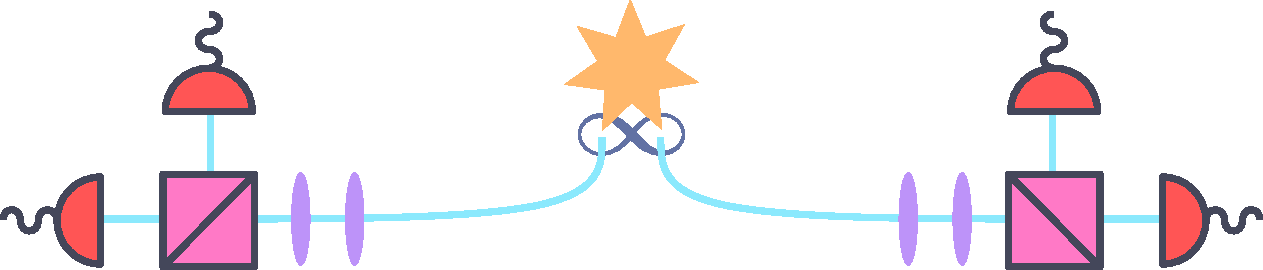
\includegraphics[width=0.95\textwidth]{chapters/deviceindependent/img/spdc.pdf}
	\end{center}
	\caption{SPDC setup. A SPDC source (yellow star) sends photons entangled in polarization (blue lines), with one part send to Alice and one send to Bob.
	Locally, each party dispose of wave plates (purple ellipse) used to chose the measurement basis according to the measurement setting. This is followed by a polarising beamsplitter (pink sliced square) with each of the two outputs measured by NPNR detectors.}
	\label{fig:spdc}
\end{figure}

\medbreak

Let us briefly described the statistics obtained from this implementation.
An SPDC source is often implemented as a laser pulsed into a non-linear crystal.
This emits photons in coupled modes, with mode $a$ send to Alice and mode $b$ send to Bob.
Note that here we only consider a single mode, whereas, in practice, multiple modes can be created.
We denote $a,a_\perp$ the two orthogonal polarizations of Alice's mode, and, similarly $b,b_\perp$ for Bob.
The state emitted is given by
\begin{equation}
	\ket{\psi} = \sqrt{1-T_g}\sqrt{1-T_{g'}}\exp(T_{g} a^\dag\,a^\dag_\perp - T_{g'}b^\dag\,b_\perp^\dag)\ket{00}
\end{equation}
with $T_g = \tanh(g)$ and $T_{g'} = \tanh(g')$, and where $g$ and $g'$ are the squeezing parameters given by the non-linear susceptibility of the crystal and by the power of the pump.

For each measurement input, Alice rotates her measurement basis with mean of wave plates.
Formally, for angles $(\alpha_x,\phi_x)$ corresponding to the input choice $x$, the two orthogonal polarization change following
\begin{equation}
	\begin{split}
		a &= \cos(\alpha_x)\tilde{a} + e^{i\phi_x}\sin(\alpha_x)\tilde{a}_\perp, \\
		a_\perp &= e^{-i\phi_x}\sin(\alpha_x)\tilde{a}-\cos(\alpha_x)\tilde{a}_\perp.
	\end{split}
\end{equation}
where $(\tilde{a},\tilde{a}_\perp)$ form a new polarization basis.
Similarly, Bob obtains a new polarization basis $(\tilde{b},\tilde{b}_\perp)$ from angles $(\beta_y,\varphi_y)$ for input $y$.

Finally, each polarizing beam-splitter outputs two-modes, on for each polarization basis, that are measured using single-photon detectors.
For Alice, the detectors will measure the modes $\tilde{a},\tilde{a}_\perp$, respectively, while for Bob they will resolve $\tilde{b}$ for one and $\tilde{b}_\perp$ for the other.
Such detectors are \acrfull{NPNR} detectors with outcomes $+1$, or \textit{click}, when a photonic signal is detected and $-1$, or \textit{no-click}, otherwise.
These detector have an efficiency $\eta$, i.e. in the presence of photons the outcome should be $+1$ with probability $\eta$.
Formally, a $\eta$-efficient NPNR detector on a mode $\tilde{a}$, is characterized by the POVM $\{M_{-1}^{\tilde{a}},1-M_{+1}^{\tilde{a}}\}$ where
\begin{equation}
	M_{-1}^{\tilde{a}} = (1-\eta)^{\tilde{a}^\dag\tilde{a}}.
\end{equation}
To obtain binary outcomes, Alice and Bob bin their four potential outcomes $\{p_H,p_V\}=\{\pm1,\pm1\}$.
For the outcomes pair $\{p_H,p_V\}$, a clever binning choice gives the outcome
\begin{equation}
	p=\begin{cases}
		+1, &\text{ if } \{p_H,p_V\}=\{+1,-1\}\\
		-1, &\text{otherwise}.
	\end{cases}
\end{equation}

Combing the expression of the state, the measurement basis choices and the detection operators, one can compute the statistics $p(ab|xy)$ as a function of the squeezing parameters, Alice and Bob measurements angles and detector efficiencies.
The full derivation of these statistics can be found in \cite{Vivoli2015b} and \cite{Ho2020}.

\medbreak

\begin{figure}[ht!]
	\begin{center}
		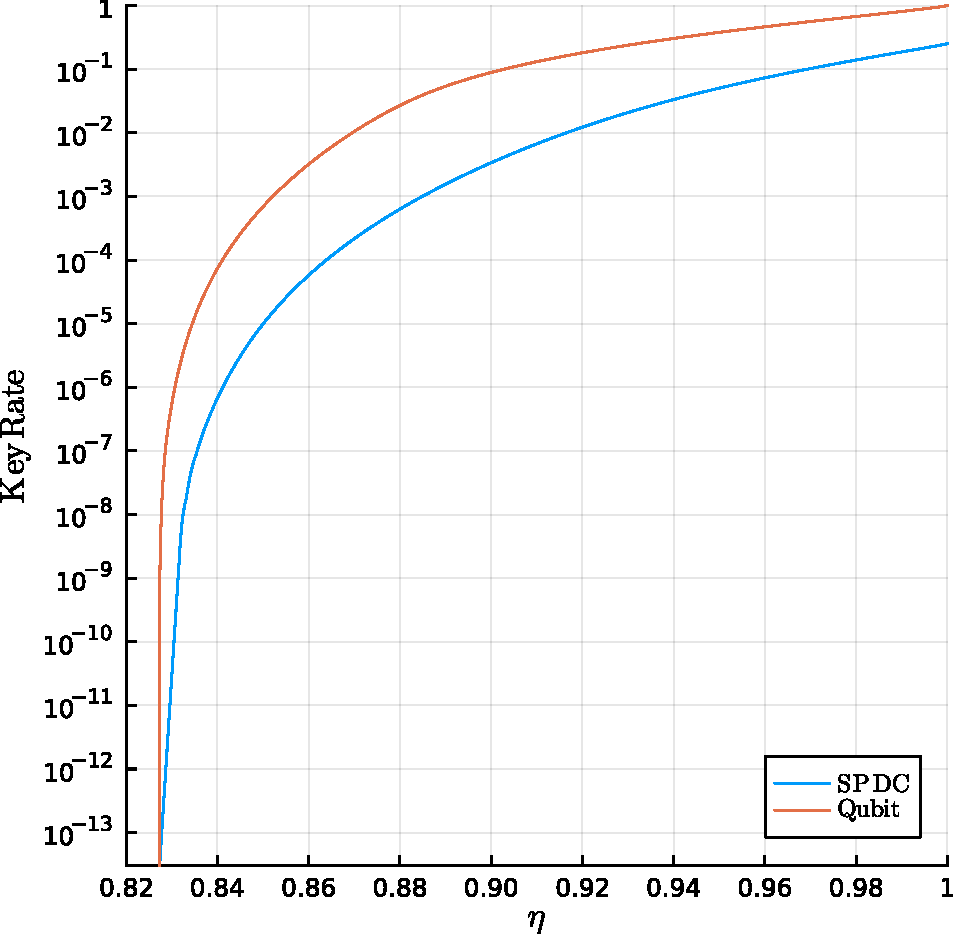
\includegraphics[width=.95\textwidth]{chapters/deviceindependent/img/key_rate_spdc.pdf}
	\end{center}
	\caption{Key rate with efficiency. The blue line correspond to the key rate obtained from a SPDC setup when all source and measurement parameters are optimized. The bump is an artifact due to a more precise optimisation performed for efficiency close the critical one. The orange curve gives the key rate obtained for two-qubit partially entangled state, as a reference.}
	\label{fig:SPDC_kr}
\end{figure}

The statistics computed from the SPDC setup allow to study its application for DIQKD.
This is achieved by optimising the key rate over the squeezing parameters and measurement angles.
With this method, we can recover the critical detection efficiency by repeating the optimisation for progressively smaller efficiency $\eta$ until no positive key rate is obtained.
Note that this possible as losses in the optical fiber before detection can be reformulate as inefficient NPRP detectors, i.e. these two types of losses commute. 
The evolution of the key rate with the detection efficiency is shown in \reffig{SPDC_kr}.

Using the key rate \refeq{Ho}, with fine-grained error correction and noisy preprocessing, the mono-mode SPDC setup have a key rate of $r\approx 0.2552$ for the ideal case $\eta=1$. 
When allowing for more modes, the key rate goes up to $\approx 0.295$.
This setup also requires a detection efficiency of at least $\eta\approx 0.826$ to yield a positive key rate.
This critical efficiency is independent on the amount of modes we consider as a difference in CHSH violation between single and multi-mode SPDC source is only noticeable for efficiency higher that $0.9$~\cite{Vivoli2015b}.


%Give key rates from Melvyn's paper.
%
%Also key rate are equivalent to two-qubit partially entangled state when considering better key rate (generalized CHSH).

\section{Automatic design of photonic experiments}

If photonic setups are a promising plateform for quantum information processing and, in particular, for DIQKD, finding a suitable photonic experiment design is cumbersome.
Indeed, thanks to integrated photonic~\cite{Pelucchi2021} there is the possibility to implement complex circuits, combining numerous optical devices.
Therefore, a systematic search through all possible implementations seems unrealistic.
Furthermore, for each photonic setup, carrying the computation either by hand is a time-consuming task while using numerical analysis based on available Fock-representation framework quickly turn resource heavy when precise computation and more optical modes are considered.
Finally, with a constant evolution of DIQKD protocols, new implementations need to be proposed continuously.

To circumvent these issues, in Article 4~\cite{Valcarce2022b}, we propose an approach using machine learning and an efficient custom-made photonic simulation framework which, together, can propose photonic design matching a given figure of merit, e.g. a DIQKD key rate. 
In the next two subsections, we give an overview of this method.
Then, we show how our method performs for the design of DIQKD experiments as well as for another figure of merit.

\begin{figure}
	\begin{center}
		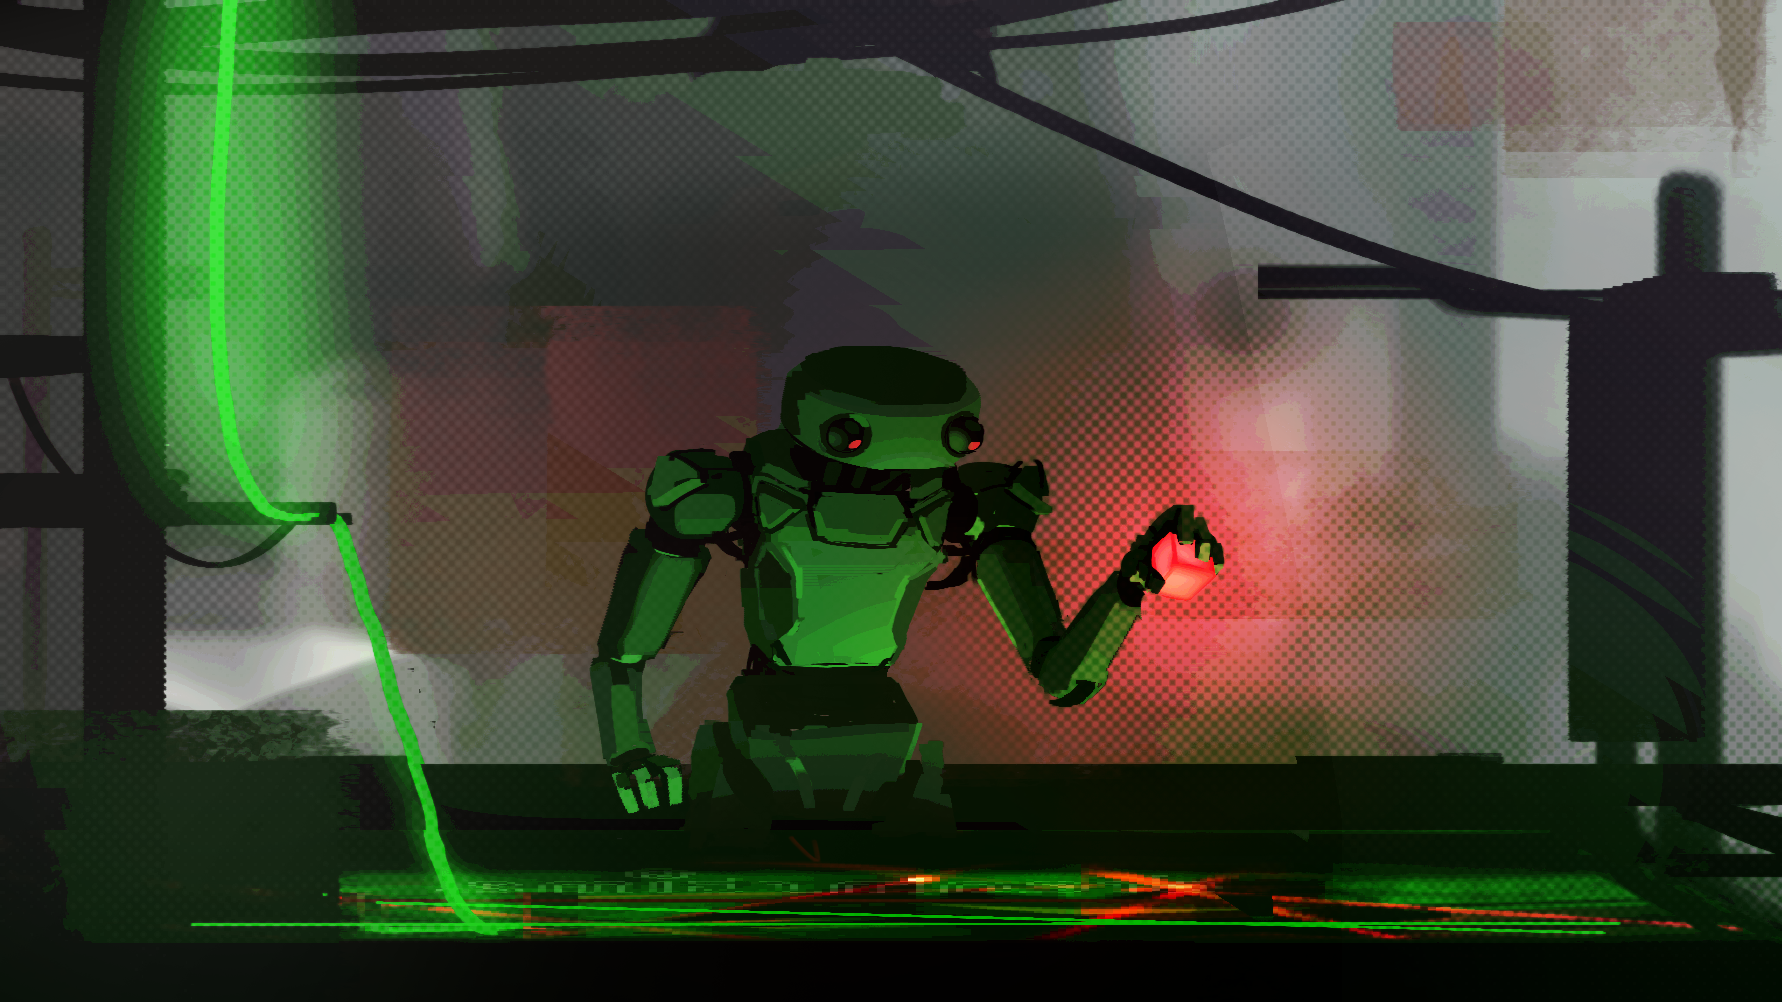
\includegraphics[width=0.95\textwidth]{chapters/deviceindependent/img/illustration_automated_design.png}
	\end{center}
	\caption{Artist's impression of the automated design of photonic experiments. \textcopyright\, Dowinson Nguyen.}
	\label{fig:}
\end{figure}



\subsection{Simulating quantum optical circuits}

Photonic circuits can be seen as a quantum circuits where each mode $i$ is a bosonic mode characterized by the bosonic operators $a_i,a_i^\dagger$, and where gates are transformations of these modes.
We restrict ourselves to optical transformation that are commonly available in quantum optics laboratory : single- and two-modes squeezers, displacements, phase-shifters and beam-splitters.
To measure these bosonic modes, we focus on non photon-number resolving (NPNR) detectors sometimes called single-photon detectors, which have outcome $+1$ or \textit{click}, when a signal is detected and $-1$, or \textit{no-click}, otherwise.
In addition to these operations, we also include heralding operations, conditioning the state of the circuit on the presence of signal in the heralded mode.


In order to efficiently explore these photonic setups, there is the need for a fast and accurate simulation framework.
Therefore, we based our approach on the Gaussian representation of state and operations, allowing for an exact and memory-efficient representation of circuits.
We then developed a numerical framework using this representation to efficiently evaluate any given photonic circuit.


\paragraph{Gaussian Quantum optics}

Consider a $n$-mode bosonic system. 
Each mode $i$ can be described in term of quadrature operators; the position $x_i=(a_i^\dagger+a_i)/2$ and the momentum $p_i=i(a_i^\dagger-a_i)/2$ operator.
The entire circuit is thus characterized by the vector $\mathbf{q}=(q_1,\dots,q_{2n})=(x_1,p_1,\dots,x_n,p_n)$.

Gaussian states, such as the vacuum state, are fully characterized by a displacement vector $\mathbf{\mu}$ and a covariance matrix $\Sigma$.
Elements of these two object are functions of $\mathbf{q}$, they are given by
\begin{align}
	\mathbf{\mu} = (\mu_1,\dots,\mu_{2n}), \qquad &\text{with}\quad \mu_i = \mean{q_i} = \trr{\rho q_i} \\
	\Sigma = \begin{pmatrix} \Sigma_{11} & \dots & \Sigma_{1,2n} \\
							\vdots & \ddots & \vdots \\
						\Sigma{2n,1} & \dots & \Sigma_{2n,2n}\end{pmatrix} , \qquad &\text{with}\quad \Sigma_{i,j} = \frac{\mean{q_i q_j + q_j q_i}}{2}-\mu_i \mu_j.
\end{align}
This representation is compact as it only need $2n(n+1)$ real parameters to fully characterized a $n$-mode bosonic system.

Gaussian transformations are transformations which conserve the Gaussian properties of Gaussian states. 
The optical devices listed above are all Gaussian transformations.
Such transformation are represented by a vector $\mathbf{d}$ of size $2n$ and by a symplectic matrix $M$ of size $2n\times2n$.
Apply on a Gaussian state $(\mathbf{\mu},\Sigma)$, such transformations output
\begin{equation}
	(\mathbf{\mu},\sigma)\; \mapsto\; (M\mathbf{\mu} + d,\, M\Sigma M^T).
\end{equation}

The no-click probability of a NPNR detector with efficiency $\eta$, on mode $i$, $p_{\circ,i}$, is computed from the displacement vector and covariance matrix of a Gaussian state following
\begin{equation}
p_{\circ i} =\frac{2}{2-\eta}\sqrt{\frac{(\det \Sigma)^{-1}}{ \det(\Sigma^{-1}+F)}}
e^{-\frac{1}{2}{\mathbf{\mu} }^T\left( \Sigma^{-1} - \Sigma^{-1} (\Sigma^{-1}+F)^{-1} \Sigma^{-1} \right){\mathbf{\mu} }}
\end{equation}
where
\begin{equation}
F= \left(\begin{array}{cc}
    \frac{4\eta}{2-\eta} & 0 \\
    0 & \frac{4\eta}{2-\eta}
    \end{array}\right)_{2i-1,2i} \oplus 0_{2n-2}.
\end{equation}
Trivially, the click probability in mode $i$ is given by $p_{\bullet,i}=1-p_{\circ,i}$.

Heralded operations are non-Gaussian operations.
However, the state $\rho_{\bullet,i}$resulting of a $n$-mode Gaussian state conditioned on a click in a mode $i$, can be expressed as a sum of two $(n-1)$-modes Gaussian state
\begin{equation}
    \rho_{\bullet,i} = \frac{\rho_{\lnot,i} - p_{\circ,i} \rho_{\circ,i}}{1 - p_{\circ,i}}
\end{equation}
where $\rho_{\lnot,i}$ is the Gaussian state with the mode $i$ traced out and where $\rho_{\circ,i}$ is the Gaussian state after a no-click event.
Therefore, with $2^{n-m}(2m^2+3m+1)$ real parameters, we can represent a $n$-mode photonic circuits undergoing $n-m$ heralding operations.

More details on the exact expression of the Gaussian transformation for each optical devices, on the expression used to obtain the statistics of joined NPNR detections, and their derivations can be found in Appendix A of Article 4.

\paragraph{QuantumOpticalCircuits.jl}

Using the Julia programming language~\cite{Bezanson2017}, we developed \textsc{QuantumOpticalCircuits.jl}, a package to simulate efficiently and accurately photonic setups~\cite{Valcarce2021}.
This package relies on the Gaussian representation to store states in a compact form and to compute accurately the effect of optical gates and the outcomes of single photon detectors.
It includes all the optical devices we listed above as well as NPNR detectors and heralded operations.

Our package makes extensive use of the multiple-dispatch paradigm of the Julia programming language.
Hence, it can easily be extended to include other operations or measurements.
Furthermore, we design this package with ease-of-use in mind, so that programming a photonic setup to be simulated becomes accessible.
Finally, even if it is less efficient, we also provide a Fock representation back-end, as this representation is more common in the community.
A simple example using this framework can be seen in \reffig{QOC.jl}.

\begin{figure}
	\begin{center}
		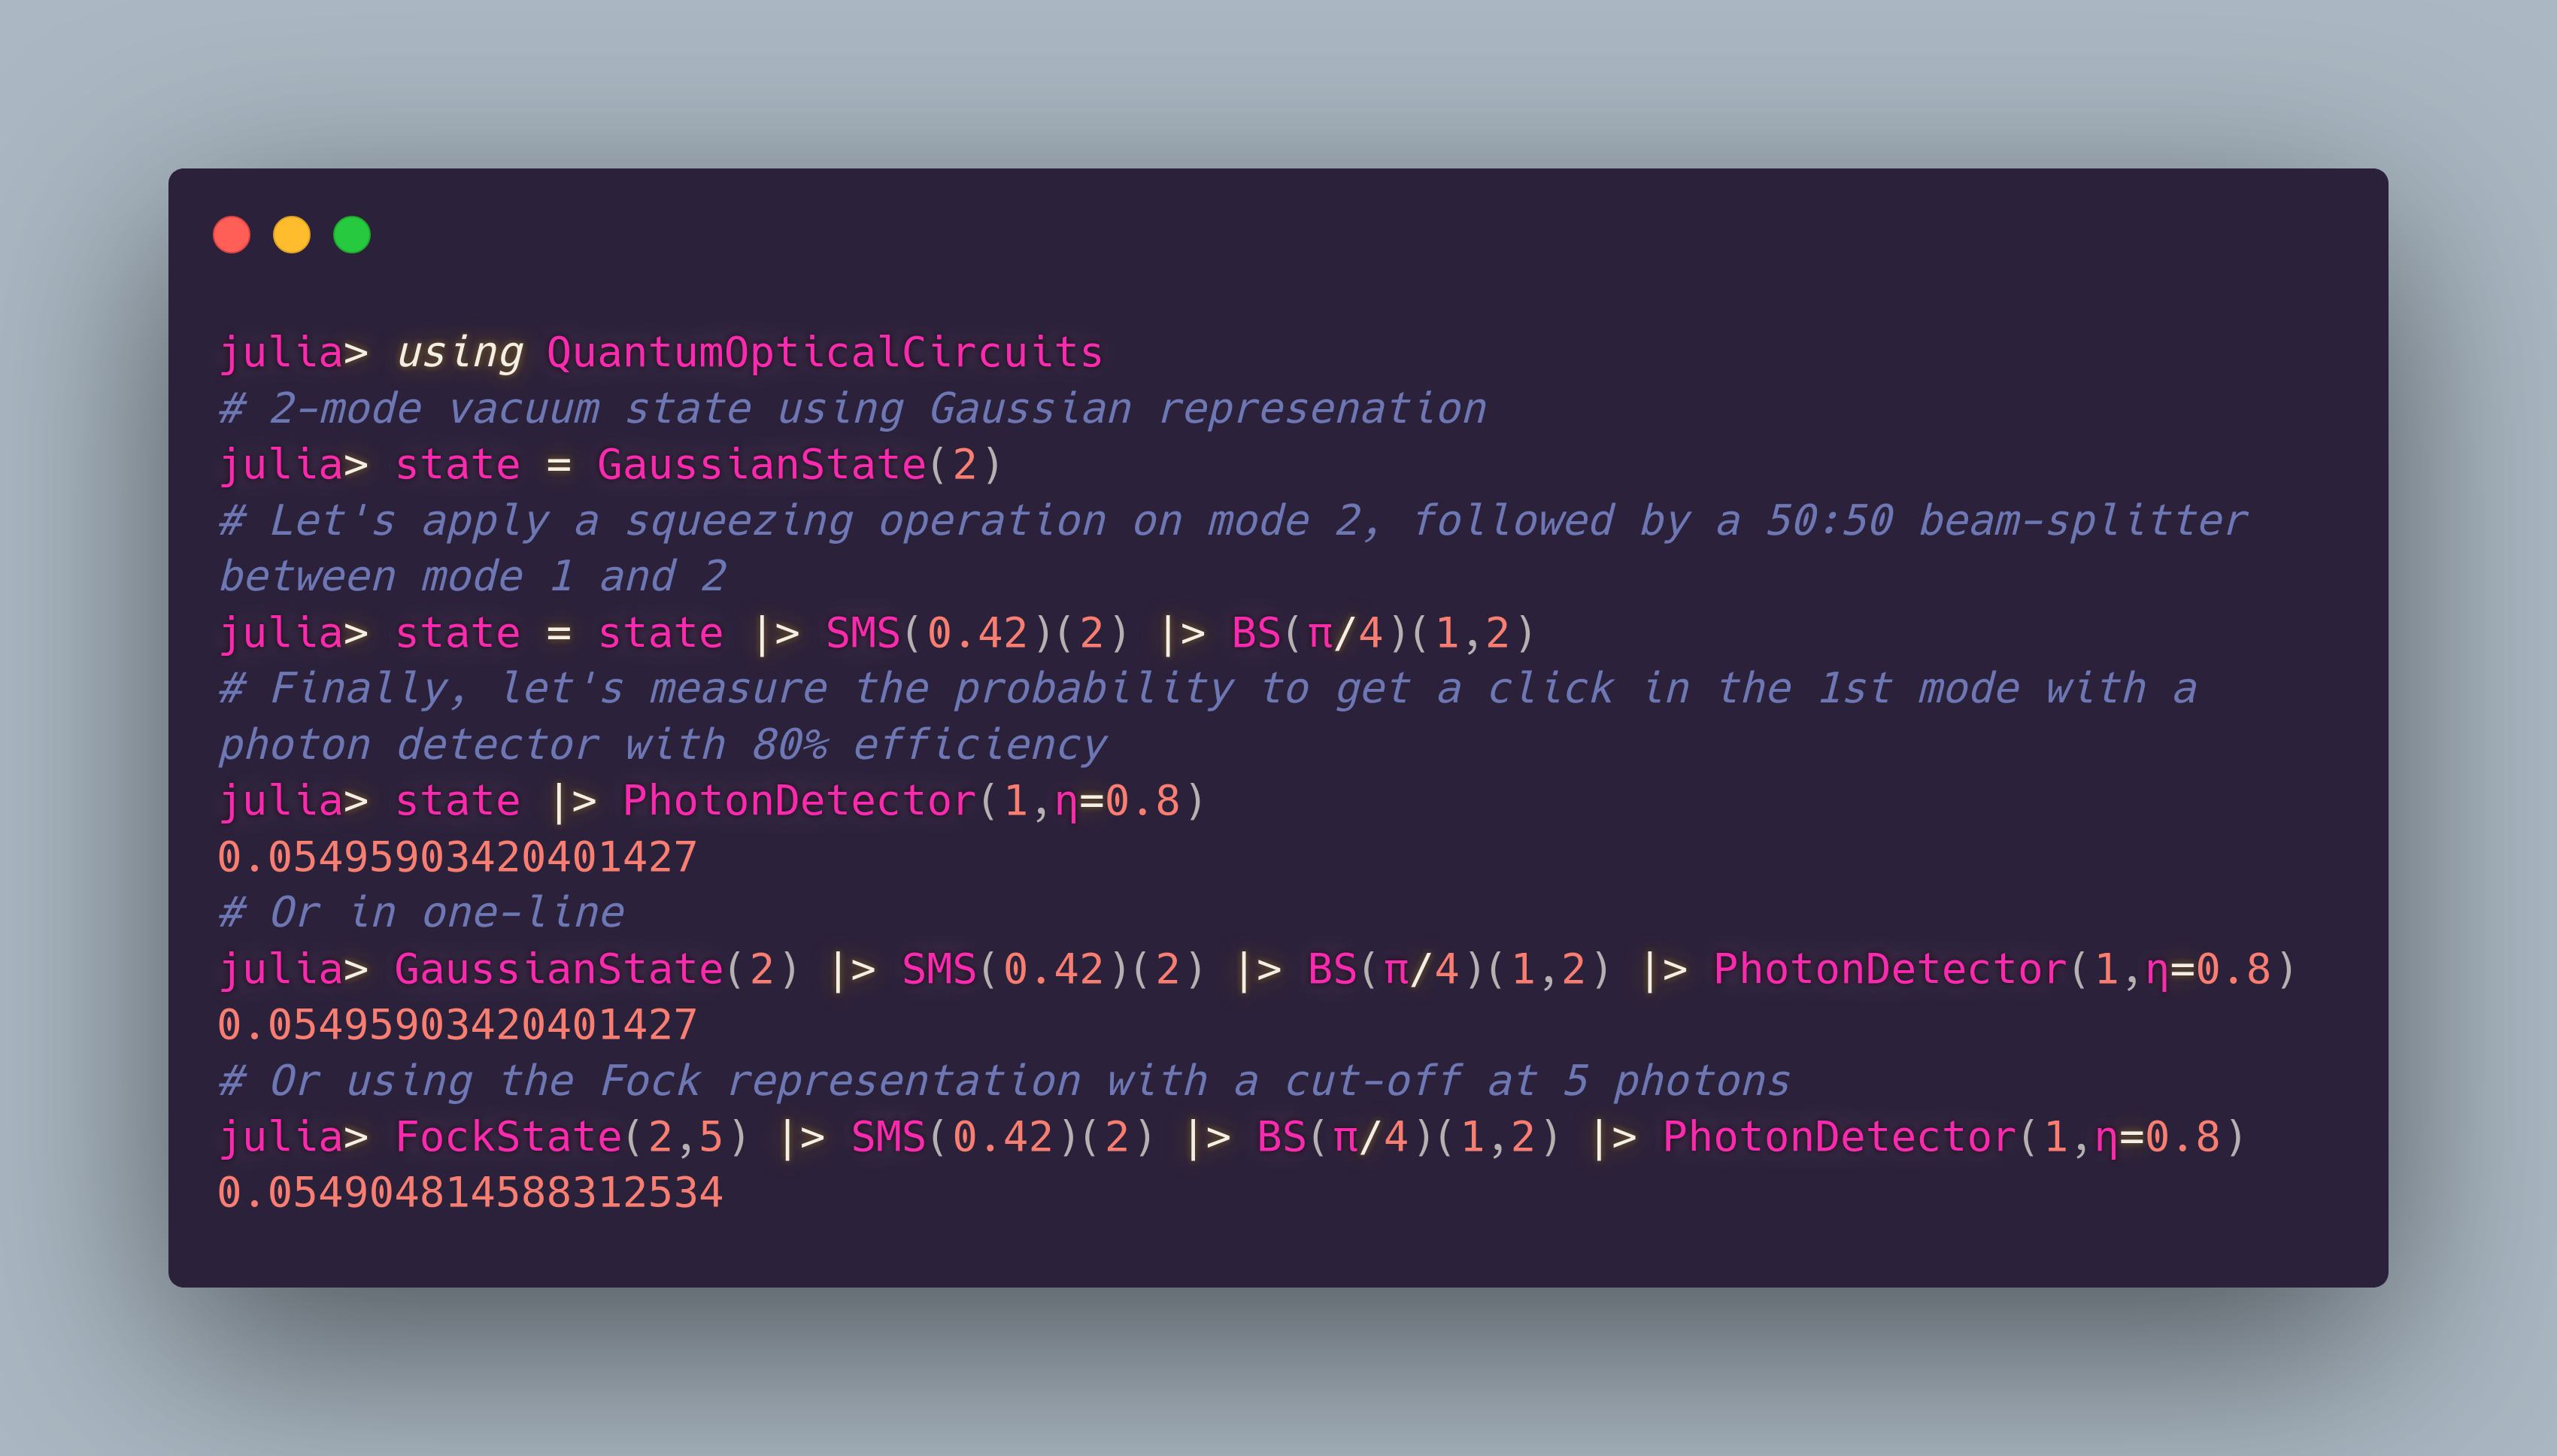
\includegraphics[width=1\textwidth]{chapters/deviceindependent/img/quantumopticalcircuits.png}
	\end{center}
	\caption{Example usage of QuantumOpticalCircuits.jl in the Julia REPL. }
	\label{fig:QOC.jl}
\end{figure}


\subsection{Reinforcement Learning}

\acrfull{rl} is a machine learning paradigm that involves an intelligent agent learning to perform a task by interacting with an environment~\cite{Sutton2018}.
Schematically, from the current state of an environment, an agent will chose an action to be performed.
Feedback is then provided in the form of the new state of the environment and a \textit{reward}, designed to quantify the quality of the action-state pair with respect to the goal task.
From this feedback, the agent updates the way actions are chosen in order to maximize the reward received. 

One of the key advantage of \acrshort{rl} is that is does not require pre-generated data to be trained on, unlike supervised and unsupervised learning.
This is particularly beneficial when generating data is costly as it is the case with the simulation of optical circuits.

\medbreak

\acrshort{rl} has seen numerous successful applications to a great variety of tasks, from learning to play games~\cite{Mnih2015,Silver2017,Vinyals2019} to finding new algorithm for matrix multiplications~\cite{Fawzi2022}.
In the field of quantum physics, \acrshort{rl} has been applied to design quantum error correction algorithms~\cite{Andreasson2019,Nautrup2019,Sweke2020}, quantum gates~\cite{Niu2019}, or new quantum experiments~\cite{Melnikov2018,Krenn2016,Krenn2020,Krenn2021}, in particular to design photonic Bell test experiments~\cite{Melnikov2020}.

Motivated by these past works, in Article 4, we proposed an approach that combine reinforcement learning and our photonic circuit simulation framework to generate new photonic experiment designs.
As an agent we use \acrfull{ppo}, a deep reinforcement learning algorithm, known to be sample efficient~\cite{Schulman2017}.
Actions that can be chosen from are optical devices that act on a specific mode or pair of modes.
After appending a chosen action to the photonic circuit, an optimization over the optical devices' parameters is run in order to maximize a given function of the statistics, e.g. a DIQKD key rate, from which the reward is computed.
From past experiences -- state, chosen action, new state and reward -- the \acrshort{ppo} algorithm updates its policy so that future chosen actions maximize the reward obtained.


\subsection{Application to DIQKD}

We applied our automated approach to the design of DIQKD experiments.
We limit ourselves to 3-modes photonic circuits with the third one being heralded before Alice and Bob's measurements.
The measurements we consider are heterodyne measurements, i.e. a displacement operation followed by a NPNR detector.

First, we picked a reward to maximize the key rate ~\refeq{Ho} achieved in an ideal scenario, i.e. in the absence of losses and noises.
After training a \acrshort{ppo} agent on that task, we obtained a fairly complex photonic circuit, composed of 12 elements.
In the ideal case, this setup achieve a key rate of $r_{Ho}\approx 0.914$, outperforming the benchmark implementation detailed in \ref{sec:PolarizationDIQKD}.
However, this setup seems not so robust to losses as we were able to obtain positive key rate for $\eta \apprge 0.874$ only.
Then, we crafted a reward to maximize the robustness of the key rate to losses.
Our method provided a simple circuit of only 7 optical devices, more robust that the reference implementation.
Indeed, this setup output key rate $r_{Ho}\geq10^{-8}$ for efficiency $\apprge 0.8245$. 
Furthermore, the obtained key rate are consistently higher that the one achieved by the benchmark setup.
These setups as well as their key rate with efficiency can be found in Article 4.


\subsection{Application toward continuous-variable DIQKD}

Our automated approach for designing photonic experiments can be readily extended to implement any task that can be expressed as a function of measurements.
An interesting task for quantum cryptography is \textit{continuous-variable} DIQKD; DIQKD implementations in which Alice and Bob perform homodyne measurements, resolving the quadratures $x,p$ of bosonic modes.
These measurements are particularly relevant as they are known to be robust to losses and can be performed at a high repetition rate.
However, if a violation of the CHSH inequality -- the first step toward DIQKD -- can be obtained in this regime, the implementation with the highest violation that has been proposed so far yield a score of $S \approx 2.046$~\cite{GarciaPatron2004,GarciaPatron2005}.
From this low violation current DIQKD protocols provide a mere positive key rates, e.g. even considering the unrealistic case of $H(A_0'|B_2)=0.0$, \refeq{Ho} gives only $r_{Ho}\approx 10^{-2}$.
To improve on this violation, a proposal combing homodyne and NPNR detectors has shown an expected violation of $S\approx 2.25$~\cite{Cavalcanti2011}.
Another proposal has shown that a Bell violation of $S \approx 2.35$ can be obtained provided that one trust the measurement devices, which is not-relevant for DIQKD~\cite{Thearle2018}.

It is in this context that we apply our automated method with the task of maximizing the CHSH violation using solely homodyne measurement, heralding operations, and the optical devices listed above.
We limit our selves to the measurement settings proposed in \cite{GarciaPatron2005} and to a sign binning of the homodyne measurement outcome.
After learning, our intelligent agent proposed the circuit depicted in \reffig{homodyne}. 
Interestingly, this circuit attain a CHSH score of $S\approx 2.068$. 
Encouragingly, this score is closed to $2.072$, the maximum violation that could be reached with homodyne measurements, sign binning and any state of the form $\ket{\psi}=\sum_i c_i \ket{i,i}$~\cite{Munro1999}.

\begin{figure}[ht]
	\begin{center}
		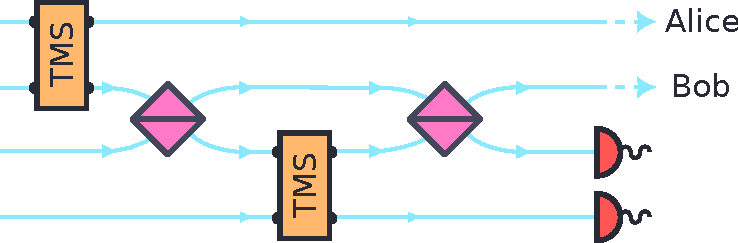
\includegraphics[width=0.95\textwidth]{chapters/deviceindependent/img/homodyne.pdf}
	\end{center}
	\caption{Circuit achieving a CHSH score $S\approx 2.068$. The blue lines are bosonic modes. The yellow rectangle labeled TMS represent two-mode squeezer, with optimal squeezing parameters $g_1=0.44689$ and $g_2=8.47\times 10^{-3}$ respectively. The two sliced pink squares are beam-splitters with optimal parameters $\theta_1 = 0.04202$ and $\theta_2 = 0.04338$. The two red half circles represent NPNR dectors heralding the modes 3 and 4. The final prepared state is post-selected on a double click, i.e. in
	both mode 3 and 4, which occurs with a probability of $p\approx 4.05\times10^{-7}$. The first mode is then send to Alice while the second is send to Bob.}
	\label{fig:homodyne}
\end{figure}





\chapter*{Article 3}
\article{Device-independent quantum key distribution from generalized CHSH inequalities}

\centering
\textrm{\LARGE Device-independent quantum key distribution from generalized CHSH inequalities}

\vspace{2cm}

\normalsize
Pavel Sekatski$^{1}$, Jean-Daniel Bancal$^{2}$, Xavier Valcarce$^{3}$, Ernest Y.-Z. Tan$^{4}$, Renato Renner$^{4}$, and Nicolas Sangouard$^{1,3}$
\bigbreak

{\footnotesize
	$^1$ Departement Physik, Universität Basel, Klingelbergstraße 82, 4056 Basel, Schweiz \\
	$^2$ Department of Applied Physics, University of Geneva, Chemin de Pinchat 22, 1211 Geneva, Switzerland \\
	$^3$ Université Paris-Saclay, CEA, CNRS, Institut de Physique Théorique, 91191 Gif-sur-Yvette, France \\
	$^4$ Institute for Theoretical Physics, ETH Zürich, 8093 Zürich, Switzerland
}

\raggedright
\bigbreak
\faLink \quad \href{https://quantum-journal.org/papers/q-2021-04-26-444/}{Quantum, volume 5, page 444} \\
\faLink \quad \href{https://arxiv.org/abs/2009.01784v4}{arXiv preprint: 2009.01784v4}
\vspace{1cm}

\centering
\textbf{Abstract}
\bigbreak

Device-independent quantum key distribution aims at providing security guarantees even when using largely uncharacterised devices.
In the simplest scenario, these guarantees are derived from the CHSH score, which is a simple linear combination of four correlation functions.
We here derive a security proof from a generalisation of the CHSH score, which effectively takes into account the individual values of two correlation functions.
We show that this additional information, which is anyway available in practice, allows one to get higher key rates than with the CHSH score.
We discuss the potential advantage of this technique for realistic photonic implementations of device-independent quantum key distribution.

\end{center}

\chapter*{Article 4}
\article{Automated design of quantum optical experiments for device-independent quantum key distribution}

\begin{center}
\textrm{\LARGE Automated design of quantum optical experiments for device-independent quantum key distribution}

\vspace{2cm}

\normalsize
Xavier Valcarce$^{1}$, Pavel Sekatski$^{2}$, Elie Gouzien$^{1}$, Alexey Melnikov$^{3}$, Nicolas Sangouard$^{1}$
\bigbreak

{\footnotesize
	$^1$ Université Paris-Saclay, CEA, CNRS, Institut de Physique Théorique, 91191 Gif-sur-Yvette, France \\
	$^2$ Department of Applied Physics, University of Geneva, Chemin de Pinchat 22, 1211 Geneva, Switzerland \\
	$^3$ Terra Quantum AG, 9000 St Gallen, Switzerland
}

\raggedright
\bigbreak
\faLink \quad \href{https://arxiv.org/abs/2209.06468}{arXiv preprint: 2209.06468}
\vspace{1cm}

\centering
\textbf{Abstract}
\bigbreak

Device-independent quantum key distribution (DIQKD) reduces the vulnerability to side-channel attacks of standard QKD protocols by removing the need for characterized quantum devices.
The higher security guarantees come however, at the price of a challenging implementation.
Here, we tackle the question of the conception of an experiment for implementing DIQKD with photonic devices.
We introduce a technique combining reinforcement learning, optimisation algorithm and a custom efficient simulation of quantum optics experiments to automate the design of photonic setups maximizing a given function of the measurement statistics.
Applying the algorithm to DIQKD, we get unexpected experimental configurations leading to high key rates and to a high resistance to loss and noise.
These configurations might be helpful to facilitate a first implementation of DIQKD with photonic devices and for future developments targeting improved performances.

\end{center}





\part{Conclusion and perspectives}

\printbibliography[heading=bibintoc]

\end{document}
